% Options for packages loaded elsewhere
\PassOptionsToPackage{unicode}{hyperref}
\PassOptionsToPackage{hyphens}{url}
%
\documentclass[
  doc,floatsintext]{apa6}
\usepackage{amsmath,amssymb}
\usepackage{iftex}
\ifPDFTeX
  \usepackage[T1]{fontenc}
  \usepackage[utf8]{inputenc}
  \usepackage{textcomp} % provide euro and other symbols
\else % if luatex or xetex
  \usepackage{unicode-math} % this also loads fontspec
  \defaultfontfeatures{Scale=MatchLowercase}
  \defaultfontfeatures[\rmfamily]{Ligatures=TeX,Scale=1}
\fi
\usepackage{lmodern}
\ifPDFTeX\else
  % xetex/luatex font selection
\fi
% Use upquote if available, for straight quotes in verbatim environments
\IfFileExists{upquote.sty}{\usepackage{upquote}}{}
\IfFileExists{microtype.sty}{% use microtype if available
  \usepackage[]{microtype}
  \UseMicrotypeSet[protrusion]{basicmath} % disable protrusion for tt fonts
}{}
\makeatletter
\@ifundefined{KOMAClassName}{% if non-KOMA class
  \IfFileExists{parskip.sty}{%
    \usepackage{parskip}
  }{% else
    \setlength{\parindent}{0pt}
    \setlength{\parskip}{6pt plus 2pt minus 1pt}}
}{% if KOMA class
  \KOMAoptions{parskip=half}}
\makeatother
\usepackage{xcolor}
\usepackage{color}
\usepackage{fancyvrb}
\newcommand{\VerbBar}{|}
\newcommand{\VERB}{\Verb[commandchars=\\\{\}]}
\DefineVerbatimEnvironment{Highlighting}{Verbatim}{commandchars=\\\{\}}
% Add ',fontsize=\small' for more characters per line
\usepackage{framed}
\definecolor{shadecolor}{RGB}{248,248,248}
\newenvironment{Shaded}{\begin{snugshade}}{\end{snugshade}}
\newcommand{\AlertTok}[1]{\textcolor[rgb]{0.94,0.16,0.16}{#1}}
\newcommand{\AnnotationTok}[1]{\textcolor[rgb]{0.56,0.35,0.01}{\textbf{\textit{#1}}}}
\newcommand{\AttributeTok}[1]{\textcolor[rgb]{0.13,0.29,0.53}{#1}}
\newcommand{\BaseNTok}[1]{\textcolor[rgb]{0.00,0.00,0.81}{#1}}
\newcommand{\BuiltInTok}[1]{#1}
\newcommand{\CharTok}[1]{\textcolor[rgb]{0.31,0.60,0.02}{#1}}
\newcommand{\CommentTok}[1]{\textcolor[rgb]{0.56,0.35,0.01}{\textit{#1}}}
\newcommand{\CommentVarTok}[1]{\textcolor[rgb]{0.56,0.35,0.01}{\textbf{\textit{#1}}}}
\newcommand{\ConstantTok}[1]{\textcolor[rgb]{0.56,0.35,0.01}{#1}}
\newcommand{\ControlFlowTok}[1]{\textcolor[rgb]{0.13,0.29,0.53}{\textbf{#1}}}
\newcommand{\DataTypeTok}[1]{\textcolor[rgb]{0.13,0.29,0.53}{#1}}
\newcommand{\DecValTok}[1]{\textcolor[rgb]{0.00,0.00,0.81}{#1}}
\newcommand{\DocumentationTok}[1]{\textcolor[rgb]{0.56,0.35,0.01}{\textbf{\textit{#1}}}}
\newcommand{\ErrorTok}[1]{\textcolor[rgb]{0.64,0.00,0.00}{\textbf{#1}}}
\newcommand{\ExtensionTok}[1]{#1}
\newcommand{\FloatTok}[1]{\textcolor[rgb]{0.00,0.00,0.81}{#1}}
\newcommand{\FunctionTok}[1]{\textcolor[rgb]{0.13,0.29,0.53}{\textbf{#1}}}
\newcommand{\ImportTok}[1]{#1}
\newcommand{\InformationTok}[1]{\textcolor[rgb]{0.56,0.35,0.01}{\textbf{\textit{#1}}}}
\newcommand{\KeywordTok}[1]{\textcolor[rgb]{0.13,0.29,0.53}{\textbf{#1}}}
\newcommand{\NormalTok}[1]{#1}
\newcommand{\OperatorTok}[1]{\textcolor[rgb]{0.81,0.36,0.00}{\textbf{#1}}}
\newcommand{\OtherTok}[1]{\textcolor[rgb]{0.56,0.35,0.01}{#1}}
\newcommand{\PreprocessorTok}[1]{\textcolor[rgb]{0.56,0.35,0.01}{\textit{#1}}}
\newcommand{\RegionMarkerTok}[1]{#1}
\newcommand{\SpecialCharTok}[1]{\textcolor[rgb]{0.81,0.36,0.00}{\textbf{#1}}}
\newcommand{\SpecialStringTok}[1]{\textcolor[rgb]{0.31,0.60,0.02}{#1}}
\newcommand{\StringTok}[1]{\textcolor[rgb]{0.31,0.60,0.02}{#1}}
\newcommand{\VariableTok}[1]{\textcolor[rgb]{0.00,0.00,0.00}{#1}}
\newcommand{\VerbatimStringTok}[1]{\textcolor[rgb]{0.31,0.60,0.02}{#1}}
\newcommand{\WarningTok}[1]{\textcolor[rgb]{0.56,0.35,0.01}{\textbf{\textit{#1}}}}
\usepackage{graphicx}
\makeatletter
\def\maxwidth{\ifdim\Gin@nat@width>\linewidth\linewidth\else\Gin@nat@width\fi}
\def\maxheight{\ifdim\Gin@nat@height>\textheight\textheight\else\Gin@nat@height\fi}
\makeatother
% Scale images if necessary, so that they will not overflow the page
% margins by default, and it is still possible to overwrite the defaults
% using explicit options in \includegraphics[width, height, ...]{}
\setkeys{Gin}{width=\maxwidth,height=\maxheight,keepaspectratio}
% Set default figure placement to htbp
\makeatletter
\def\fps@figure{htbp}
\makeatother
\setlength{\emergencystretch}{3em} % prevent overfull lines
\providecommand{\tightlist}{%
  \setlength{\itemsep}{0pt}\setlength{\parskip}{0pt}}
\setcounter{secnumdepth}{-\maxdimen} % remove section numbering
% Make \paragraph and \subparagraph free-standing
\makeatletter
\ifx\paragraph\undefined\else
  \let\oldparagraph\paragraph
  \renewcommand{\paragraph}{
    \@ifstar
      \xxxParagraphStar
      \xxxParagraphNoStar
  }
  \newcommand{\xxxParagraphStar}[1]{\oldparagraph*{#1}\mbox{}}
  \newcommand{\xxxParagraphNoStar}[1]{\oldparagraph{#1}\mbox{}}
\fi
\ifx\subparagraph\undefined\else
  \let\oldsubparagraph\subparagraph
  \renewcommand{\subparagraph}{
    \@ifstar
      \xxxSubParagraphStar
      \xxxSubParagraphNoStar
  }
  \newcommand{\xxxSubParagraphStar}[1]{\oldsubparagraph*{#1}\mbox{}}
  \newcommand{\xxxSubParagraphNoStar}[1]{\oldsubparagraph{#1}\mbox{}}
\fi
\makeatother
\ifLuaTeX
\usepackage[bidi=basic]{babel}
\else
\usepackage[bidi=default]{babel}
\fi
\babelprovide[main,import]{english}
% get rid of language-specific shorthands (see #6817):
\let\LanguageShortHands\languageshorthands
\def\languageshorthands#1{}
% Manuscript styling
\usepackage{upgreek}
\captionsetup{font=singlespacing,justification=justified}

% Table formatting
\usepackage{longtable}
\usepackage{lscape}
% \usepackage[counterclockwise]{rotating}   % Landscape page setup for large tables
\usepackage{multirow}		% Table styling
\usepackage{tabularx}		% Control Column width
\usepackage[flushleft]{threeparttable}	% Allows for three part tables with a specified notes section
\usepackage{threeparttablex}            % Lets threeparttable work with longtable

% Create new environments so endfloat can handle them
% \newenvironment{ltable}
%   {\begin{landscape}\centering\begin{threeparttable}}
%   {\end{threeparttable}\end{landscape}}
\newenvironment{lltable}{\begin{landscape}\centering\begin{ThreePartTable}}{\end{ThreePartTable}\end{landscape}}

% Enables adjusting longtable caption width to table width
% Solution found at http://golatex.de/longtable-mit-caption-so-breit-wie-die-tabelle-t15767.html
\makeatletter
\newcommand\LastLTentrywidth{1em}
\newlength\longtablewidth
\setlength{\longtablewidth}{1in}
\newcommand{\getlongtablewidth}{\begingroup \ifcsname LT@\roman{LT@tables}\endcsname \global\longtablewidth=0pt \renewcommand{\LT@entry}[2]{\global\advance\longtablewidth by ##2\relax\gdef\LastLTentrywidth{##2}}\@nameuse{LT@\roman{LT@tables}} \fi \endgroup}

% \setlength{\parindent}{0.5in}
% \setlength{\parskip}{0pt plus 0pt minus 0pt}

% Overwrite redefinition of paragraph and subparagraph by the default LaTeX template
% See https://github.com/crsh/papaja/issues/292
\makeatletter
\renewcommand{\paragraph}{\@startsection{paragraph}{4}{\parindent}%
  {0\baselineskip \@plus 0.2ex \@minus 0.2ex}%
  {-1em}%
  {\normalfont\normalsize\bfseries\itshape\typesectitle}}

\renewcommand{\subparagraph}[1]{\@startsection{subparagraph}{5}{1em}%
  {0\baselineskip \@plus 0.2ex \@minus 0.2ex}%
  {-\z@\relax}%
  {\normalfont\normalsize\itshape\hspace{\parindent}{#1}\textit{\addperi}}{\relax}}
\makeatother

\makeatletter
\usepackage{etoolbox}
\patchcmd{\maketitle}
  {\section{\normalfont\normalsize\abstractname}}
  {\section*{\normalfont\normalsize\abstractname}}
  {}{\typeout{Failed to patch abstract.}}
\patchcmd{\maketitle}
  {\section{\protect\normalfont{\@title}}}
  {\section*{\protect\normalfont{\@title}}}
  {}{\typeout{Failed to patch title.}}
\makeatother

\usepackage{xpatch}
\makeatletter
\xapptocmd\appendix
  {\xapptocmd\section
    {\addcontentsline{toc}{section}{\appendixname\ifoneappendix\else~\theappendix\fi\\: #1}}
    {}{\InnerPatchFailed}%
  }
{}{\PatchFailed}
\usepackage{lineno}

\linenumbers
\usepackage{csquotes}
\ifLuaTeX
  \usepackage{selnolig}  % disable illegal ligatures
\fi
\usepackage{bookmark}
\IfFileExists{xurl.sty}{\usepackage{xurl}}{} % add URL line breaks if available
\urlstyle{same}
\hypersetup{
  pdftitle={Experiment 2 Analysis},
  pdflang={en-EN},
  hidelinks,
  pdfcreator={LaTeX via pandoc}}

\title{Experiment 2 Analysis}
\author{\phantom{0}}
\date{}


\shorttitle{Revised Exp 2}

\affiliation{\phantom{0}}

\begin{document}
\maketitle

\subsection{Experiment 2: Honorific Greetings}\label{experiment-2-honorific-greetings}

\subsubsection{Participants}\label{participants}

\begin{Shaded}
\begin{Highlighting}[]
\NormalTok{g\_fin }\OtherTok{\textless{}{-}} \FunctionTok{read.csv}\NormalTok{(}\FunctionTok{here}\NormalTok{(}\StringTok{\textquotesingle{}data/greetings\_reviewer2\_data.csv\textquotesingle{}}\NormalTok{))}
\NormalTok{g\_fin}\SpecialCharTok{$}\NormalTok{subject\_id }\OtherTok{\textless{}{-}} \FunctionTok{as.factor}\NormalTok{(g\_fin}\SpecialCharTok{$}\NormalTok{subject\_id)}

\NormalTok{g\_pp\_tab }\OtherTok{\textless{}{-}}\NormalTok{ g\_fin }\SpecialCharTok{\%\textgreater{}\%} 
  \FunctionTok{distinct}\NormalTok{(subject\_id, bebe\_meses)}\SpecialCharTok{\%\textgreater{}\%} 
  \FunctionTok{summarize}\NormalTok{(}\AttributeTok{min=}\FunctionTok{min}\NormalTok{(bebe\_meses),}
            \AttributeTok{max=}\FunctionTok{max}\NormalTok{(bebe\_meses),}
            \AttributeTok{M=}\FunctionTok{mean}\NormalTok{(bebe\_meses),}
            \AttributeTok{SD=}\FunctionTok{sd}\NormalTok{(bebe\_meses))}

\NormalTok{G\_N }\OtherTok{\textless{}{-}} \FunctionTok{nrow}\NormalTok{(g\_fin }\SpecialCharTok{\%\textgreater{}\%} 
  \FunctionTok{distinct}\NormalTok{(subject\_id, bebe\_meses))}
\NormalTok{G\_MIN\_AGE }\OtherTok{\textless{}{-}} \FunctionTok{op}\NormalTok{(g\_pp\_tab}\SpecialCharTok{$}\NormalTok{min)}
\NormalTok{G\_MAX\_AGE }\OtherTok{\textless{}{-}} \FunctionTok{op}\NormalTok{(g\_pp\_tab}\SpecialCharTok{$}\NormalTok{max)}
\NormalTok{G\_MEAN\_AGE }\OtherTok{\textless{}{-}} \FunctionTok{op}\NormalTok{(g\_pp\_tab}\SpecialCharTok{$}\NormalTok{M)}
\NormalTok{G\_SD\_AGE }\OtherTok{\textless{}{-}} \FunctionTok{op}\NormalTok{(g\_pp\_tab}\SpecialCharTok{$}\NormalTok{SD)}
\end{Highlighting}
\end{Shaded}

\begin{Shaded}
\begin{Highlighting}[]
\NormalTok{g\_mama\_tab }\OtherTok{\textless{}{-}}\NormalTok{ demo }\SpecialCharTok{\%\textgreater{}\%}
  \FunctionTok{filter}\NormalTok{(subject\_id }\SpecialCharTok{\%in\%}\NormalTok{ g\_fin}\SpecialCharTok{$}\NormalTok{subject\_id,}
         \SpecialCharTok{!}\FunctionTok{is.na}\NormalTok{(mama\_edad)) }\SpecialCharTok{\%\textgreater{}\%}
  \FunctionTok{summarize}\NormalTok{(}\AttributeTok{min=}\FunctionTok{min}\NormalTok{(mama\_edad),}
            \AttributeTok{max=}\FunctionTok{max}\NormalTok{(mama\_edad),}
            \AttributeTok{M=}\FunctionTok{mean}\NormalTok{(mama\_edad),}
            \AttributeTok{SD=}\FunctionTok{sd}\NormalTok{(mama\_edad))}

\NormalTok{G\_MOT\_MIN\_AGE }\OtherTok{\textless{}{-}} \FunctionTok{op}\NormalTok{(g\_mama\_tab}\SpecialCharTok{$}\NormalTok{min)}
\NormalTok{G\_MOT\_MAX\_AGE }\OtherTok{\textless{}{-}} \FunctionTok{op}\NormalTok{(g\_mama\_tab}\SpecialCharTok{$}\NormalTok{max)}
\NormalTok{G\_MOT\_M\_AGE }\OtherTok{\textless{}{-}} \FunctionTok{op}\NormalTok{(g\_mama\_tab}\SpecialCharTok{$}\NormalTok{M)}
\NormalTok{G\_MOT\_SD\_AGE }\OtherTok{\textless{}{-}} \FunctionTok{op}\NormalTok{(g\_mama\_tab}\SpecialCharTok{$}\NormalTok{SD)}
\end{Highlighting}
\end{Shaded}

We report on data from \(18\) infants (\textit{range}\(=5.33-14.93\)\textit{mos}, \(M_\textnormal{age}=10.77\)\textit{mos}, \(SD_\textnormal{age}=2.67\)\textit{mos}) tested in the Canada Chica \textit{paraje} of a Tseltal Maya community in Tenejapa, Chiapas, in Southern Mexico.

Mothers ranged in age from \(14.00\) to \(42.00\)\textit{yrs} (\(M_\textnormal{age}=26.81\)\textit{yrs}, \(SD_\textnormal{age}=7.80\)\textit{yrs})

\subsubsection{Mean Difference Score Analysis}\label{mean-difference-score-analysis}

\begin{Shaded}
\begin{Highlighting}[]
\NormalTok{g\_fin}\SpecialCharTok{$}\NormalTok{stimulus\_set }\OtherTok{\textless{}{-}} \StringTok{\textquotesingle{}\textquotesingle{}}

\NormalTok{g\_fin[g\_fin}\SpecialCharTok{$}\NormalTok{old\_trial\_name }\SpecialCharTok{\%in\%} \FunctionTok{c}\NormalTok{(}\StringTok{\textquotesingle{}old\_woman{-}YOUNG\_MAN\textquotesingle{}}\NormalTok{,}
                          \StringTok{\textquotesingle{}OLD\_WOMAN{-}young\_man\textquotesingle{}}\NormalTok{), ]}\SpecialCharTok{$}\NormalTok{stimulus\_set }\OtherTok{\textless{}{-}} \StringTok{\textquotesingle{}A\textquotesingle{}}

\NormalTok{g\_fin[g\_fin}\SpecialCharTok{$}\NormalTok{old\_trial\_name }\SpecialCharTok{\%in\%} \FunctionTok{c}\NormalTok{(}\StringTok{\textquotesingle{}young\_man{-}OLD\_WOMAN\textquotesingle{}}\NormalTok{,}
                          \StringTok{\textquotesingle{}YOUNG\_MAN{-}old\_woman\textquotesingle{}}\NormalTok{), ]}\SpecialCharTok{$}\NormalTok{stimulus\_set }\OtherTok{\textless{}{-}} \StringTok{\textquotesingle{}B\textquotesingle{}}

\NormalTok{g\_fin[g\_fin}\SpecialCharTok{$}\NormalTok{old\_trial\_name }\SpecialCharTok{\%in\%} \FunctionTok{c}\NormalTok{(}\StringTok{\textquotesingle{}old\_man{-}YOUNG\_WOMAN\textquotesingle{}}\NormalTok{,}
                          \StringTok{\textquotesingle{}OLD\_MAN{-}young\_woman\textquotesingle{}}\NormalTok{), ]}\SpecialCharTok{$}\NormalTok{stimulus\_set }\OtherTok{\textless{}{-}} \StringTok{\textquotesingle{}C\textquotesingle{}}

\NormalTok{g\_fin[g\_fin}\SpecialCharTok{$}\NormalTok{old\_trial\_name }\SpecialCharTok{\%in\%} \FunctionTok{c}\NormalTok{(}\StringTok{\textquotesingle{}young\_woman{-}OLD\_MAN\textquotesingle{}}\NormalTok{,}
                          \StringTok{\textquotesingle{}YOUNG\_WOMAN{-}old\_man\textquotesingle{}}\NormalTok{), ]}\SpecialCharTok{$}\NormalTok{stimulus\_set }\OtherTok{\textless{}{-}} \StringTok{\textquotesingle{}D\textquotesingle{}}

\NormalTok{g\_fin}\SpecialCharTok{$}\NormalTok{target\_stimulus }\OtherTok{\textless{}{-}} \FunctionTok{paste}\NormalTok{(g\_fin}\SpecialCharTok{$}\NormalTok{target\_noun, g\_fin}\SpecialCharTok{$}\NormalTok{stimulus\_set, }\AttributeTok{sep=}\StringTok{\textquotesingle{}\textquotesingle{}}\NormalTok{)}
\NormalTok{g\_fin}\SpecialCharTok{$}\NormalTok{non\_target\_stimulus }\OtherTok{\textless{}{-}} \StringTok{\textquotesingle{}\textquotesingle{}}

\NormalTok{g\_fin[g\_fin}\SpecialCharTok{$}\NormalTok{target\_stimulus}\SpecialCharTok{==}\StringTok{\textquotesingle{}young\_manA\textquotesingle{}}\NormalTok{,]}\SpecialCharTok{$}\NormalTok{non\_target\_stimulus }\OtherTok{\textless{}{-}} \StringTok{\textquotesingle{}old\_womanA\textquotesingle{}}
\NormalTok{g\_fin[g\_fin}\SpecialCharTok{$}\NormalTok{target\_stimulus}\SpecialCharTok{==}\StringTok{\textquotesingle{}old\_womanA\textquotesingle{}}\NormalTok{,]}\SpecialCharTok{$}\NormalTok{non\_target\_stimulus }\OtherTok{\textless{}{-}} \StringTok{\textquotesingle{}young\_manA\textquotesingle{}}

\NormalTok{g\_fin[g\_fin}\SpecialCharTok{$}\NormalTok{target\_stimulus}\SpecialCharTok{==}\StringTok{\textquotesingle{}young\_manB\textquotesingle{}}\NormalTok{,]}\SpecialCharTok{$}\NormalTok{non\_target\_stimulus }\OtherTok{\textless{}{-}} \StringTok{\textquotesingle{}old\_womanB\textquotesingle{}}
\NormalTok{g\_fin[g\_fin}\SpecialCharTok{$}\NormalTok{target\_stimulus}\SpecialCharTok{==}\StringTok{\textquotesingle{}old\_womanB\textquotesingle{}}\NormalTok{,]}\SpecialCharTok{$}\NormalTok{non\_target\_stimulus }\OtherTok{\textless{}{-}} \StringTok{\textquotesingle{}young\_manB\textquotesingle{}}

\NormalTok{g\_fin[g\_fin}\SpecialCharTok{$}\NormalTok{target\_stimulus}\SpecialCharTok{==}\StringTok{\textquotesingle{}young\_womanC\textquotesingle{}}\NormalTok{,]}\SpecialCharTok{$}\NormalTok{non\_target\_stimulus }\OtherTok{\textless{}{-}} \StringTok{\textquotesingle{}old\_manC\textquotesingle{}}
\NormalTok{g\_fin[g\_fin}\SpecialCharTok{$}\NormalTok{target\_stimulus}\SpecialCharTok{==}\StringTok{\textquotesingle{}old\_manC\textquotesingle{}}\NormalTok{,]}\SpecialCharTok{$}\NormalTok{non\_target\_stimulus }\OtherTok{\textless{}{-}} \StringTok{\textquotesingle{}young\_womanC\textquotesingle{}}

\NormalTok{g\_fin[g\_fin}\SpecialCharTok{$}\NormalTok{target\_stimulus}\SpecialCharTok{==}\StringTok{\textquotesingle{}young\_womanD\textquotesingle{}}\NormalTok{,]}\SpecialCharTok{$}\NormalTok{non\_target\_stimulus }\OtherTok{\textless{}{-}} \StringTok{\textquotesingle{}old\_manD\textquotesingle{}}
\NormalTok{g\_fin[g\_fin}\SpecialCharTok{$}\NormalTok{target\_stimulus}\SpecialCharTok{==}\StringTok{\textquotesingle{}old\_manD\textquotesingle{}}\NormalTok{,]}\SpecialCharTok{$}\NormalTok{non\_target\_stimulus }\OtherTok{\textless{}{-}} \StringTok{\textquotesingle{}young\_womanD\textquotesingle{}}

\NormalTok{g\_target\_df }\OtherTok{\textless{}{-}}\NormalTok{ g\_fin }\SpecialCharTok{\%\textgreater{}\%}
  \FunctionTok{filter}\NormalTok{(noun\_pair }\SpecialCharTok{\%in\%} \FunctionTok{c}\NormalTok{(}\StringTok{\textquotesingle{}old\_man{-}young\_woman\textquotesingle{}}\NormalTok{, }\StringTok{\textquotesingle{}old\_woman{-}young\_man\textquotesingle{}}\NormalTok{),}
\NormalTok{         subject\_id }\SpecialCharTok{\%in\%}\NormalTok{ g\_subjects) }\SpecialCharTok{\%\textgreater{}\%}
\NormalTok{  dplyr}\SpecialCharTok{::}\FunctionTok{select}\NormalTok{(subject\_id, }
\NormalTok{                bebe\_meses,}
\NormalTok{                age\_centered,}
\NormalTok{                age\_group,}
\NormalTok{                stimulus\_set, }
\NormalTok{                target\_stimulus, }
\NormalTok{                noun\_pair, }
\NormalTok{                post1\_target\_prop) }\SpecialCharTok{\%\textgreater{}\%}
  \FunctionTok{mutate}\NormalTok{(}\AttributeTok{merge\_on\_noun =}\NormalTok{ target\_stimulus)}

\NormalTok{g\_non\_target\_df }\OtherTok{\textless{}{-}}\NormalTok{ g\_fin }\SpecialCharTok{\%\textgreater{}\%}
  \FunctionTok{filter}\NormalTok{(noun\_pair }\SpecialCharTok{\%in\%} \FunctionTok{c}\NormalTok{(}\StringTok{\textquotesingle{}old\_man{-}young\_woman\textquotesingle{}}\NormalTok{, }\StringTok{\textquotesingle{}old\_woman{-}young\_man\textquotesingle{}}\NormalTok{),}
\NormalTok{                          subject\_id }\SpecialCharTok{\%in\%}\NormalTok{ g\_subjects) }\SpecialCharTok{\%\textgreater{}\%}
\NormalTok{  dplyr}\SpecialCharTok{::}\FunctionTok{select}\NormalTok{(subject\_id, }
\NormalTok{                bebe\_meses,}
\NormalTok{                age\_centered,}
\NormalTok{                age\_group,}
\NormalTok{                noun\_pair,}
\NormalTok{                stimulus\_set, }
\NormalTok{                non\_target\_stimulus,}
\NormalTok{                post1\_nontarget\_prop) }\SpecialCharTok{\%\textgreater{}\%}
  \FunctionTok{mutate}\NormalTok{(}\AttributeTok{merge\_on\_noun=}\NormalTok{non\_target\_stimulus)}

\NormalTok{g\_target\_nontarget\_props\_df }\OtherTok{\textless{}{-}} \FunctionTok{merge}\NormalTok{(g\_target\_df, g\_non\_target\_df, }
                                      \AttributeTok{by=}\FunctionTok{c}\NormalTok{(}\StringTok{\textquotesingle{}subject\_id\textquotesingle{}}\NormalTok{, }
                                           \StringTok{\textquotesingle{}noun\_pair\textquotesingle{}}\NormalTok{,}
                                           \StringTok{\textquotesingle{}stimulus\_set\textquotesingle{}}\NormalTok{,}
                                           \StringTok{\textquotesingle{}merge\_on\_noun\textquotesingle{}}\NormalTok{,}
                                           \StringTok{\textquotesingle{}age\_centered\textquotesingle{}}\NormalTok{,}
                                           \StringTok{\textquotesingle{}bebe\_meses\textquotesingle{}}\NormalTok{,}
                                           \StringTok{\textquotesingle{}age\_group\textquotesingle{}}\NormalTok{), }\AttributeTok{all=}\NormalTok{T) }\SpecialCharTok{\%\textgreater{}\%}
  \FunctionTok{group\_by}\NormalTok{(subject\_id, bebe\_meses, age\_centered, age\_group,}
\NormalTok{           noun\_pair, stimulus\_set, merge\_on\_noun) }\SpecialCharTok{\%\textgreater{}\%}
  \FunctionTok{summarize}\NormalTok{(}\AttributeTok{post1\_target\_prop =} \FunctionTok{na.mean}\NormalTok{(post1\_target\_prop),}
            \AttributeTok{post1\_nontarget\_prop =} \FunctionTok{na.mean}\NormalTok{(post1\_nontarget\_prop))}

\NormalTok{g\_diffs\_df }\OtherTok{\textless{}{-}}\NormalTok{  g\_target\_nontarget\_props\_df }\SpecialCharTok{\%\textgreater{}\%}
\NormalTok{  dplyr}\SpecialCharTok{::}\FunctionTok{select}\NormalTok{(subject\_id, bebe\_meses, age\_centered, age\_group,}
\NormalTok{                noun\_pair, stimulus\_set, merge\_on\_noun, }
\NormalTok{                post1\_target\_prop,}
\NormalTok{                post1\_nontarget\_prop) }\SpecialCharTok{\%\textgreater{}\%}
  \FunctionTok{mutate}\NormalTok{(}\AttributeTok{diff =}\NormalTok{ post1\_target\_prop }\SpecialCharTok{{-}}\NormalTok{ post1\_nontarget\_prop) }\SpecialCharTok{\%\textgreater{}\%}
  \FunctionTok{group\_by}\NormalTok{(subject\_id, }
\NormalTok{           bebe\_meses, age\_centered, age\_group, }
\NormalTok{           noun\_pair, stimulus\_set) }\SpecialCharTok{\%\textgreater{}\%}
  \FunctionTok{summarize}\NormalTok{(}\AttributeTok{stim\_pair\_diff =} \FunctionTok{mean}\NormalTok{(diff)) }\SpecialCharTok{\%\textgreater{}\%}
  \FunctionTok{group\_by}\NormalTok{(subject\_id, bebe\_meses, age\_centered, age\_group, noun\_pair) }\SpecialCharTok{\%\textgreater{}\%}
  \FunctionTok{summarize}\NormalTok{(}\AttributeTok{noun\_pair\_diff =} \FunctionTok{na.mean}\NormalTok{(stim\_pair\_diff)) }\SpecialCharTok{\%\textgreater{}\%}
         \FunctionTok{filter}\NormalTok{(}\SpecialCharTok{!}\FunctionTok{is.na}\NormalTok{(noun\_pair))}

\NormalTok{g\_diffs\_df}\SpecialCharTok{$}\NormalTok{age\_std }\OtherTok{\textless{}{-}}\NormalTok{ g\_diffs\_df}\SpecialCharTok{$}\NormalTok{age\_centered}\SpecialCharTok{/}\FunctionTok{as.numeric}\NormalTok{(G\_SD\_AGE)}

\FunctionTok{write.csv}\NormalTok{(g\_diffs\_df,}
         \FunctionTok{here}\NormalTok{(}\StringTok{\textquotesingle{}data/r\_analysis\_dfs\textquotesingle{}}\NormalTok{, }\StringTok{\textquotesingle{}g\_bs2012\_diffs.csv\textquotesingle{}}\NormalTok{)}
\NormalTok{         )}
\end{Highlighting}
\end{Shaded}

\paragraph{By Item}\label{by-item}

\begin{Shaded}
\begin{Highlighting}[]
\FunctionTok{set.seed}\NormalTok{(}\DecValTok{36}\NormalTok{)}

\NormalTok{g\_by\_item\_tab }\OtherTok{\textless{}{-}}\NormalTok{ g\_diffs\_df }\SpecialCharTok{\%\textgreater{}\%} 
  \FunctionTok{group\_by}\NormalTok{(noun\_pair, subject\_id, age\_centered) }\SpecialCharTok{\%\textgreater{}\%}
  \FunctionTok{summarize}\NormalTok{(}\AttributeTok{subj\_item\_mean =} \FunctionTok{na.mean}\NormalTok{(noun\_pair\_diff)) }\SpecialCharTok{\%\textgreater{}\%}
  \FunctionTok{filter}\NormalTok{(}\SpecialCharTok{!}\FunctionTok{is.na}\NormalTok{(subj\_item\_mean)) }\SpecialCharTok{\%\textgreater{}\%}
  \FunctionTok{ungroup}\NormalTok{() }\SpecialCharTok{\%\textgreater{}\%}
  \FunctionTok{group\_by}\NormalTok{(noun\_pair) }\SpecialCharTok{\%\textgreater{}\%}
  \FunctionTok{summarize}\NormalTok{(}\AttributeTok{n =} \FunctionTok{n}\NormalTok{(),}
            \AttributeTok{M =} \FunctionTok{na.mean}\NormalTok{(subj\_item\_mean),}
            \AttributeTok{cil=}\NormalTok{M}\SpecialCharTok{{-}}\FunctionTok{ci.low}\NormalTok{(subj\_item\_mean),}
            \AttributeTok{cih =}\NormalTok{ M}\SpecialCharTok{+}\FunctionTok{ci.high}\NormalTok{(subj\_item\_mean),}
            \AttributeTok{min=}\FunctionTok{min}\NormalTok{(subj\_item\_mean, }\AttributeTok{na.rm=}\NormalTok{T),}
            \AttributeTok{max=}\FunctionTok{max}\NormalTok{(subj\_item\_mean, }\AttributeTok{na.rm=}\NormalTok{T))}

\NormalTok{G\_ALL\_ITEM\_MEAN }\OtherTok{\textless{}{-}} \FunctionTok{mean}\NormalTok{(g\_by\_item\_tab}\SpecialCharTok{$}\NormalTok{M)}
\NormalTok{G\_ALL\_ITEM\_CIL }\OtherTok{\textless{}{-}}\NormalTok{ G\_ALL\_ITEM\_MEAN }\SpecialCharTok{{-}} \FunctionTok{ci.low}\NormalTok{(g\_by\_item\_tab}\SpecialCharTok{$}\NormalTok{M)}
\NormalTok{G\_ALL\_ITEM\_CIH }\OtherTok{\textless{}{-}}\NormalTok{ G\_ALL\_ITEM\_MEAN }\SpecialCharTok{+} \FunctionTok{ci.high}\NormalTok{(g\_by\_item\_tab}\SpecialCharTok{$}\NormalTok{M)}
\NormalTok{G\_ALL\_ITEM\_MIN }\OtherTok{\textless{}{-}} \FunctionTok{min}\NormalTok{(g\_by\_item\_tab}\SpecialCharTok{$}\NormalTok{M)}
\NormalTok{G\_ALL\_ITEM\_MAX }\OtherTok{\textless{}{-}} \FunctionTok{max}\NormalTok{(g\_by\_item\_tab}\SpecialCharTok{$}\NormalTok{M)}
\NormalTok{N\_G\_POSITIVE\_ITEMS }\OtherTok{\textless{}{-}} \FunctionTok{sum}\NormalTok{(g\_by\_item\_tab}\SpecialCharTok{$}\NormalTok{M }\SpecialCharTok{\textgreater{}} \DecValTok{0}\NormalTok{)}
\end{Highlighting}
\end{Shaded}

\begin{Shaded}
\begin{Highlighting}[]
\FunctionTok{set.seed}\NormalTok{(}\DecValTok{36}\NormalTok{)}

\FunctionTok{write}\NormalTok{(}\FunctionTok{apa\_table}\NormalTok{(g\_by\_item\_tab, }
                \AttributeTok{caption=}\StringTok{\textquotesingle{}Experiment 2 Item Means\textquotesingle{}}\NormalTok{),}
      \FunctionTok{here}\NormalTok{(}\StringTok{\textquotesingle{}supplement/tables/exp\_2/g\_by\_item\_tab.tex\textquotesingle{}}\NormalTok{))}

\FunctionTok{xtable2kable}\NormalTok{(g\_by\_item\_tab)}
\end{Highlighting}
\end{Shaded}

\begin{verbatim}
## # A tibble: 2 x 7
##   noun_pair               n      M     cil   cih    min   max
##   <chr>               <int>  <dbl>   <dbl> <dbl>  <dbl> <dbl>
## 1 old_man-young_woman    13 0.0848 -0.138  0.285 -0.713 0.538
## 2 old_woman-young_man    15 0.182   0.0648 0.305 -0.191 0.540
\end{verbatim}

\paragraph{Non-parametric}\label{non-parametric}

\begin{Shaded}
\begin{Highlighting}[]
\CommentTok{\# Bayes factor}
\FunctionTok{ttestBF}\NormalTok{(g\_by\_item\_tab}\SpecialCharTok{$}\NormalTok{M)}
\end{Highlighting}
\end{Shaded}

\begin{verbatim}
## Bayes factor analysis
## --------------
## [1] Alt., r=0.707 : 1.2 ±0%
## 
## Against denominator:
##   Null, mu = 0 
## ---
## Bayes factor type: BFoneSample, JZS
\end{verbatim}

\begin{Shaded}
\begin{Highlighting}[]
\CommentTok{\# Standard deviation}
\NormalTok{stdev}\OtherTok{=}\FunctionTok{sd}\NormalTok{(g\_by\_item\_tab}\SpecialCharTok{$}\NormalTok{M, }\AttributeTok{na.rm=}\NormalTok{T)}
\CommentTok{\# Mean}
\NormalTok{mean\_data}\OtherTok{=}\FunctionTok{na.mean}\NormalTok{(g\_by\_item\_tab}\SpecialCharTok{$}\NormalTok{M)}
\CommentTok{\# Effect size}
\NormalTok{G\_ITEM\_D}\OtherTok{=}\FunctionTok{abs}\NormalTok{(mean\_data}\SpecialCharTok{/}\NormalTok{stdev)}
\end{Highlighting}
\end{Shaded}

\begin{Shaded}
\begin{Highlighting}[]
\NormalTok{g\_by\_item\_sub\_tab }\OtherTok{\textless{}{-}}\NormalTok{ g\_diffs\_df }\SpecialCharTok{\%\textgreater{}\%} 
  \FunctionTok{group\_by}\NormalTok{(noun\_pair, subject\_id) }\SpecialCharTok{\%\textgreater{}\%}
  \FunctionTok{summarize}\NormalTok{(}\AttributeTok{subj\_item\_mean =} \FunctionTok{na.mean}\NormalTok{(noun\_pair\_diff)) }\SpecialCharTok{\%\textgreater{}\%}
  \FunctionTok{ungroup}\NormalTok{() }\SpecialCharTok{\%\textgreater{}\%}
  \FunctionTok{filter}\NormalTok{(}\SpecialCharTok{!}\FunctionTok{is.na}\NormalTok{(subj\_item\_mean)) }

\NormalTok{g\_item\_wilcox }\OtherTok{\textless{}{-}} \FunctionTok{wilcox.test}\NormalTok{(g\_by\_item\_sub\_tab}\SpecialCharTok{$}\NormalTok{subj\_item\_mean,}
                             \AttributeTok{mu=}\DecValTok{0}\NormalTok{, }
                             \AttributeTok{alternative=}\StringTok{"two.sided"}\NormalTok{)}

\NormalTok{G\_ITEM\_P\_WILCOX }\OtherTok{\textless{}{-}} \FunctionTok{reportP}\NormalTok{(}\FunctionTok{as.numeric}\NormalTok{(g\_item\_wilcox[}\StringTok{\textquotesingle{}p.value\textquotesingle{}}\NormalTok{]))}
\end{Highlighting}
\end{Shaded}

\begin{Shaded}
\begin{Highlighting}[]
\NormalTok{g\_item\_binom }\OtherTok{\textless{}{-}} \FunctionTok{binom.test}\NormalTok{(}\DecValTok{2}\NormalTok{, }\DecValTok{2}\NormalTok{, }\AttributeTok{p=}\NormalTok{.}\DecValTok{5}\NormalTok{)}

\NormalTok{G\_ITEM\_P\_BINOM }\OtherTok{\textless{}{-}} \FunctionTok{reportP}\NormalTok{(g\_item\_binom}\SpecialCharTok{$}\NormalTok{p.value)}
\end{Highlighting}
\end{Shaded}

\begin{Shaded}
\begin{Highlighting}[]
\FunctionTok{set.seed}\NormalTok{(}\DecValTok{36}\NormalTok{)}

\NormalTok{g\_diffs\_df}\SpecialCharTok{$}\NormalTok{noun\_pair\_label }\OtherTok{\textless{}{-}} \StringTok{\textquotesingle{}\textquotesingle{}}
\NormalTok{g\_diffs\_df[}
\NormalTok{  g\_diffs\_df}\SpecialCharTok{$}\NormalTok{noun\_pair}\SpecialCharTok{==}\StringTok{\textquotesingle{}old\_woman{-}young\_man\textquotesingle{}}\NormalTok{,]}\SpecialCharTok{$}\NormalTok{noun\_pair\_label }\OtherTok{\textless{}{-}}
  \StringTok{\textquotesingle{}old woman {-}}\SpecialCharTok{\textbackslash{}n}\StringTok{young man\textquotesingle{}}
\NormalTok{g\_diffs\_df[}
\NormalTok{  g\_diffs\_df}\SpecialCharTok{$}\NormalTok{noun\_pair}\SpecialCharTok{==}\StringTok{\textquotesingle{}old\_man{-}young\_woman\textquotesingle{}}\NormalTok{,]}\SpecialCharTok{$}\NormalTok{noun\_pair\_label }\OtherTok{\textless{}{-}}
  \StringTok{\textquotesingle{}old man {-}}\SpecialCharTok{\textbackslash{}n}\StringTok{young woman\textquotesingle{}}

\NormalTok{g\_plot2 }\OtherTok{\textless{}{-}}\NormalTok{ g\_diffs\_df }\SpecialCharTok{\%\textgreater{}\%} 
  \FunctionTok{group\_by}\NormalTok{(noun\_pair, noun\_pair\_label, subject\_id) }\SpecialCharTok{\%\textgreater{}\%}
  \FunctionTok{summarize}\NormalTok{(}\AttributeTok{subj\_item\_mean =} \FunctionTok{na.mean}\NormalTok{(noun\_pair\_diff)) }\SpecialCharTok{\%\textgreater{}\%}
  \FunctionTok{ungroup}\NormalTok{() }\SpecialCharTok{\%\textgreater{}\%}
  \FunctionTok{filter}\NormalTok{(}\SpecialCharTok{!}\FunctionTok{is.na}\NormalTok{(subj\_item\_mean)) }\SpecialCharTok{\%\textgreater{}\%}
  \FunctionTok{group\_by}\NormalTok{(noun\_pair, noun\_pair\_label) }\SpecialCharTok{\%\textgreater{}\%}
  \FunctionTok{mutate}\NormalTok{(}\AttributeTok{n =} \FunctionTok{n}\NormalTok{(),}
            \AttributeTok{item\_mean =} \FunctionTok{na.mean}\NormalTok{(subj\_item\_mean),}
            \AttributeTok{min=}\FunctionTok{min}\NormalTok{(subj\_item\_mean, }\AttributeTok{na.rm=}\NormalTok{T),}
            \AttributeTok{max=}\FunctionTok{max}\NormalTok{(subj\_item\_mean, }\AttributeTok{na.rm=}\NormalTok{T),}
            \AttributeTok{ci.low=}\NormalTok{item\_mean}\SpecialCharTok{{-}}\FunctionTok{ci.low}\NormalTok{(subj\_item\_mean),}
            \AttributeTok{ci.high =}\NormalTok{ item\_mean}\SpecialCharTok{+}\FunctionTok{ci.high}\NormalTok{(subj\_item\_mean)) }\SpecialCharTok{\%\textgreater{}\%}
  \FunctionTok{ggplot}\NormalTok{(., }\FunctionTok{aes}\NormalTok{(}\AttributeTok{x=}\NormalTok{noun\_pair\_label, }\AttributeTok{y=}\NormalTok{item\_mean, }\AttributeTok{color=}\NormalTok{noun\_pair)) }\SpecialCharTok{+}
    \FunctionTok{geom\_hline}\NormalTok{(}\AttributeTok{yintercept=}\DecValTok{0}\NormalTok{) }\SpecialCharTok{+}
  \FunctionTok{geom\_jitter}\NormalTok{(}\FunctionTok{aes}\NormalTok{(}\AttributeTok{y=}\NormalTok{subj\_item\_mean), }\AttributeTok{alpha=}\NormalTok{.}\DecValTok{5}\NormalTok{) }\SpecialCharTok{+}
  \FunctionTok{geom\_pointrange}\NormalTok{(}\FunctionTok{aes}\NormalTok{(}\AttributeTok{y=}\NormalTok{item\_mean, }\AttributeTok{ymin=}\NormalTok{ci.low, }\AttributeTok{ymax=}\NormalTok{ci.high, }
                      \AttributeTok{fill=}\NormalTok{noun\_pair), }\AttributeTok{shape=}\DecValTok{23}\NormalTok{, }\AttributeTok{size=}\NormalTok{.}\DecValTok{5}\NormalTok{) }\SpecialCharTok{+} 
\NormalTok{  sb.density.theme }\SpecialCharTok{+}
  \FunctionTok{theme}\NormalTok{(}\AttributeTok{axis.text.x =} \FunctionTok{element\_text}\NormalTok{(}\AttributeTok{angle=}\DecValTok{60}\NormalTok{, }\AttributeTok{vjust=}\DecValTok{1}\NormalTok{, }\AttributeTok{hjust=}\DecValTok{1}\NormalTok{, }\AttributeTok{size=}\DecValTok{10}\NormalTok{),}
        \AttributeTok{legend.position =} \StringTok{"none"}\NormalTok{,}
        \AttributeTok{axis.title =} \FunctionTok{element\_text}\NormalTok{(}\AttributeTok{colour=}\StringTok{"gray30"}\NormalTok{, }\AttributeTok{size=}\DecValTok{11}\NormalTok{, }\AttributeTok{face=}\StringTok{"bold"}\NormalTok{)) }\SpecialCharTok{+}
  \FunctionTok{ylab}\NormalTok{(}\StringTok{"Increase in Target Looking"}\NormalTok{) }\SpecialCharTok{+}
  \FunctionTok{xlab}\NormalTok{(}\StringTok{"Honorific{-}Pair"}\NormalTok{) }\SpecialCharTok{+}
  \FunctionTok{ylim}\NormalTok{(}\SpecialCharTok{{-}}\DecValTok{1}\NormalTok{, }\DecValTok{1}\NormalTok{) }\SpecialCharTok{+} 
  \FunctionTok{scale\_discrete\_manual}\NormalTok{(}\AttributeTok{aesthetics=}\FunctionTok{c}\NormalTok{(}\StringTok{"color"}\NormalTok{, }\StringTok{"fill"}\NormalTok{), }
                        \AttributeTok{values=}\NormalTok{greeting\_pair\_fills)}
\end{Highlighting}
\end{Shaded}

\paragraph{By Subject}\label{by-subject}

\begin{Shaded}
\begin{Highlighting}[]
\FunctionTok{set.seed}\NormalTok{(}\DecValTok{36}\NormalTok{)}

\NormalTok{g\_sub\_df }\OtherTok{\textless{}{-}}\NormalTok{ g\_diffs\_df }\SpecialCharTok{\%\textgreater{}\%} 
  \FunctionTok{filter}\NormalTok{(}\SpecialCharTok{!}\FunctionTok{is.na}\NormalTok{(noun\_pair\_diff)) }\SpecialCharTok{\%\textgreater{}\%}
  \FunctionTok{group\_by}\NormalTok{(subject\_id, bebe\_meses, age\_centered) }\SpecialCharTok{\%\textgreater{}\%}
  \FunctionTok{summarize}\NormalTok{(}\AttributeTok{g\_M =} \FunctionTok{na.mean}\NormalTok{(noun\_pair\_diff),}
            \AttributeTok{n=}\FunctionTok{n}\NormalTok{()) }

\NormalTok{G\_N\_FOR\_MEAN\_DIFF\_ANALYSES }\OtherTok{\textless{}{-}} \FunctionTok{nrow}\NormalTok{(g\_sub\_df)}

\NormalTok{g\_positive\_scorers\_age\_tab }\OtherTok{\textless{}{-}}\NormalTok{ g\_sub\_df }\SpecialCharTok{\%\textgreater{}\%}
  \FunctionTok{filter}\NormalTok{(g\_M}\SpecialCharTok{\textgreater{}}\DecValTok{0}\NormalTok{) }\SpecialCharTok{\%\textgreater{}\%}
  \FunctionTok{ungroup}\NormalTok{() }\SpecialCharTok{\%\textgreater{}\%}
  \FunctionTok{summarize}\NormalTok{(}\AttributeTok{mean=}\FunctionTok{mean}\NormalTok{(bebe\_meses),}
            \AttributeTok{sd=}\FunctionTok{sd}\NormalTok{(bebe\_meses),}
            \AttributeTok{ci.low=}\NormalTok{mean}\SpecialCharTok{{-}}\FunctionTok{ci.low}\NormalTok{(bebe\_meses),}
            \AttributeTok{ci.high=}\NormalTok{mean}\SpecialCharTok{+}\FunctionTok{ci.high}\NormalTok{(bebe\_meses))}

\NormalTok{G\_N\_POSITIVE\_SUBS }\OtherTok{\textless{}{-}} \FunctionTok{sum}\NormalTok{(g\_sub\_df}\SpecialCharTok{$}\NormalTok{g\_M}\SpecialCharTok{\textgreater{}}\DecValTok{0}\NormalTok{)}
\NormalTok{G\_N\_TOTAL\_SUBS }\OtherTok{\textless{}{-}} \FunctionTok{nrow}\NormalTok{(g\_sub\_df)}
\NormalTok{G\_PS\_MEAN\_AGE }\OtherTok{\textless{}{-}}\NormalTok{ g\_positive\_scorers\_age\_tab}\SpecialCharTok{$}\NormalTok{mean}
\NormalTok{G\_PS\_CILO\_AGE }\OtherTok{\textless{}{-}}\NormalTok{ g\_positive\_scorers\_age\_tab}\SpecialCharTok{$}\NormalTok{ci.low}
\NormalTok{G\_PS\_CIHI\_AGE }\OtherTok{\textless{}{-}}\NormalTok{ g\_positive\_scorers\_age\_tab}\SpecialCharTok{$}\NormalTok{ci.high}
\NormalTok{G\_PS\_SD\_AGE }\OtherTok{\textless{}{-}}\NormalTok{ g\_positive\_scorers\_age\_tab}\SpecialCharTok{$}\NormalTok{sd}
\end{Highlighting}
\end{Shaded}

\begin{Shaded}
\begin{Highlighting}[]
\FunctionTok{set.seed}\NormalTok{(}\DecValTok{36}\NormalTok{)}

\NormalTok{ g\_by\_sub\_overall\_tab }\OtherTok{\textless{}{-}}\NormalTok{ g\_diffs\_df }\SpecialCharTok{\%\textgreater{}\%}
  \FunctionTok{group\_by}\NormalTok{(subject\_id) }\SpecialCharTok{\%\textgreater{}\%}
  \FunctionTok{summarize}\NormalTok{(}\AttributeTok{subj\_mean =} \FunctionTok{na.mean}\NormalTok{(noun\_pair\_diff)) }\SpecialCharTok{\%\textgreater{}\%}
  \FunctionTok{ungroup}\NormalTok{() }\SpecialCharTok{\%\textgreater{}\%}
  \FunctionTok{filter}\NormalTok{(}\SpecialCharTok{!}\FunctionTok{is.na}\NormalTok{(subj\_mean)) }\SpecialCharTok{\%\textgreater{}\%}
  \FunctionTok{summarize}\NormalTok{(}\AttributeTok{group\_subject\_mean =} \FunctionTok{mean}\NormalTok{(subj\_mean),}
            \AttributeTok{min=}\FunctionTok{min}\NormalTok{(subj\_mean),}
            \AttributeTok{max=}\FunctionTok{max}\NormalTok{(subj\_mean),}
            \AttributeTok{ci.low=}\NormalTok{group\_subject\_mean}\SpecialCharTok{{-}}\FunctionTok{ci.low}\NormalTok{(subj\_mean),}
            \AttributeTok{ci.high =}\NormalTok{ group\_subject\_mean}\SpecialCharTok{+}\FunctionTok{ci.high}\NormalTok{(subj\_mean))}

\NormalTok{G\_ALL\_SUB\_MEAN }\OtherTok{\textless{}{-}}\NormalTok{ g\_by\_sub\_overall\_tab}\SpecialCharTok{$}\NormalTok{group\_subject\_mean}
\NormalTok{G\_ALL\_SUB\_CIL }\OtherTok{\textless{}{-}}\NormalTok{ g\_by\_sub\_overall\_tab}\SpecialCharTok{$}\NormalTok{ci.low}
\NormalTok{G\_ALL\_SUB\_CIH }\OtherTok{\textless{}{-}}\NormalTok{ g\_by\_sub\_overall\_tab}\SpecialCharTok{$}\NormalTok{ci.high}
\NormalTok{G\_ALL\_SUB\_MIN }\OtherTok{\textless{}{-}}\NormalTok{ g\_by\_sub\_overall\_tab}\SpecialCharTok{$}\NormalTok{min}
\NormalTok{G\_ALL\_SUB\_MAX }\OtherTok{\textless{}{-}}\NormalTok{ g\_by\_sub\_overall\_tab}\SpecialCharTok{$}\NormalTok{max}
\end{Highlighting}
\end{Shaded}

\begin{Shaded}
\begin{Highlighting}[]
\NormalTok{g\_diffs\_df }\SpecialCharTok{\%\textgreater{}\%} 
  \FunctionTok{filter}\NormalTok{(}\SpecialCharTok{!}\FunctionTok{is.na}\NormalTok{(noun\_pair\_diff)) }\SpecialCharTok{\%\textgreater{}\%}
  \FunctionTok{group\_by}\NormalTok{(subject\_id, bebe\_meses) }\SpecialCharTok{\%\textgreater{}\%}
  \FunctionTok{summarize}\NormalTok{(}\AttributeTok{subj\_item\_mean =} \FunctionTok{na.mean}\NormalTok{(noun\_pair\_diff),}
            \AttributeTok{n\_items =} \FunctionTok{n}\NormalTok{()) }\SpecialCharTok{\%\textgreater{}\%}
  \FunctionTok{mutate}\NormalTok{(}\AttributeTok{all\_pairs =}\NormalTok{ n\_items}\SpecialCharTok{==}\DecValTok{2}\NormalTok{) }\SpecialCharTok{\%\textgreater{}\%}
  \FunctionTok{filter}\NormalTok{(}\SpecialCharTok{!}\FunctionTok{is.na}\NormalTok{(subj\_item\_mean)) }\SpecialCharTok{\%\textgreater{}\%}
\FunctionTok{ggplot}\NormalTok{(.) }\SpecialCharTok{+}
  \FunctionTok{geom\_point}\NormalTok{(}\FunctionTok{aes}\NormalTok{(}\AttributeTok{x=}\NormalTok{bebe\_meses, }\AttributeTok{y=}\NormalTok{subj\_item\_mean), }
             \AttributeTok{color=}\NormalTok{rf\_color, }\AttributeTok{fill=}\NormalTok{rf\_fill, }
             \AttributeTok{shape=}\DecValTok{24}\NormalTok{, }\AttributeTok{size=}\FloatTok{2.5}\NormalTok{) }\SpecialCharTok{+} 
  \FunctionTok{geom\_linerange}\NormalTok{(}\FunctionTok{aes}\NormalTok{(}\AttributeTok{x=}\NormalTok{bebe\_meses, }\AttributeTok{ymin=}\DecValTok{0}\NormalTok{, }\AttributeTok{ymax=}\NormalTok{subj\_item\_mean),}
                 \AttributeTok{color=}\NormalTok{rf\_color) }\SpecialCharTok{+}
  \FunctionTok{geom\_hline}\NormalTok{(}\AttributeTok{yintercept=}\DecValTok{0}\NormalTok{) }\SpecialCharTok{+}
\NormalTok{  sb.density.theme }\SpecialCharTok{+}
  \FunctionTok{theme}\NormalTok{(}
    \AttributeTok{axis.title =} \FunctionTok{element\_text}\NormalTok{(}\AttributeTok{colour=}\StringTok{"gray30"}\NormalTok{, }\AttributeTok{size=}\DecValTok{11}\NormalTok{, }\AttributeTok{face=}\StringTok{"bold"}\NormalTok{),}
        \AttributeTok{axis.text =} \FunctionTok{element\_text}\NormalTok{(}\AttributeTok{colour=}\StringTok{"gray30"}\NormalTok{, }\AttributeTok{size=}\DecValTok{11}\NormalTok{),}
        \AttributeTok{axis.ticks =} \FunctionTok{element\_line}\NormalTok{(}\AttributeTok{colour=}\StringTok{"gray30"}\NormalTok{)) }\SpecialCharTok{+}
  \FunctionTok{ylab}\NormalTok{(}\StringTok{"Increase in Target Looking"}\NormalTok{) }\SpecialCharTok{+}
  \FunctionTok{xlab}\NormalTok{(}\StringTok{"Child Age (months)"}\NormalTok{) }\SpecialCharTok{+}
  \FunctionTok{xlim}\NormalTok{(}\FloatTok{4.5}\NormalTok{, }\FloatTok{16.0}\NormalTok{) }\SpecialCharTok{+}
  \FunctionTok{scale\_x\_continuous}\NormalTok{(}\AttributeTok{breaks=}\FunctionTok{c}\NormalTok{(}\DecValTok{4}\NormalTok{,}\DecValTok{5}\NormalTok{,}\DecValTok{6}\NormalTok{,}\DecValTok{7}\NormalTok{,}\DecValTok{8}\NormalTok{,}\DecValTok{9}\NormalTok{,}\DecValTok{10}\NormalTok{,}\DecValTok{11}\NormalTok{,}\DecValTok{12}\NormalTok{,}\DecValTok{13}\NormalTok{,}\DecValTok{14}\NormalTok{,}\DecValTok{15}\NormalTok{)) }\SpecialCharTok{+}
  \FunctionTok{ylim}\NormalTok{(}\SpecialCharTok{{-}}\NormalTok{.}\DecValTok{4}\NormalTok{, .}\DecValTok{6}\NormalTok{) }
\end{Highlighting}
\end{Shaded}

\begin{figure}

{\centering 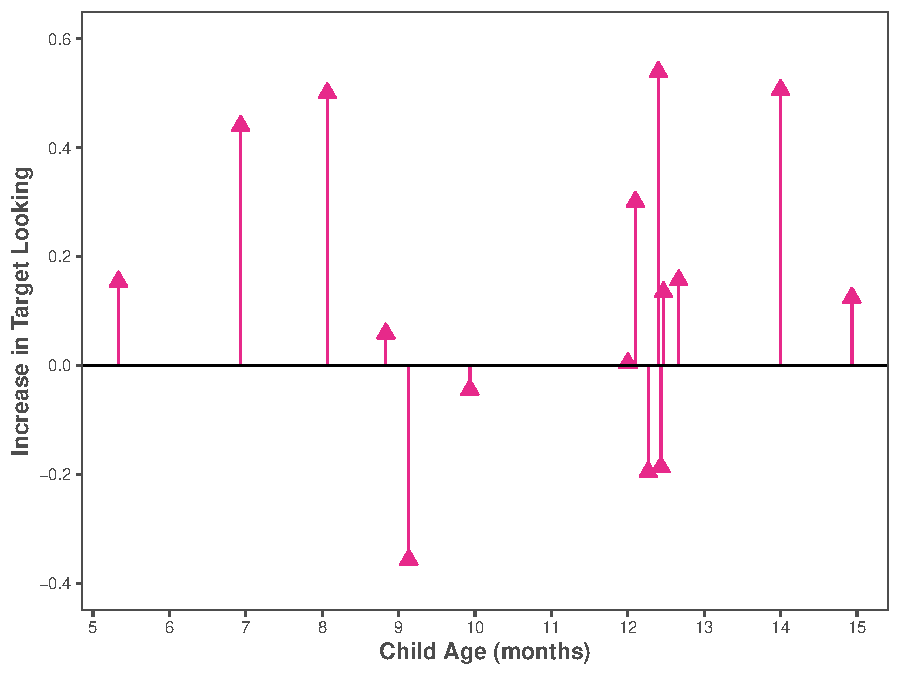
\includegraphics{revised_ms_analyses_files/figure-latex/r2-g-by-subject-plot-1} 

}

\caption{ }\label{fig:r2-g-by-subject-plot}
\end{figure}

\begin{Shaded}
\begin{Highlighting}[]
\FunctionTok{ggsave}\NormalTok{(}\FunctionTok{here}\NormalTok{(}\StringTok{\textquotesingle{}supplement/plots/exp\_2/pdfs\textquotesingle{}}\NormalTok{, }\StringTok{\textquotesingle{}g\_meandiffs\_bysub.pdf\textquotesingle{}}\NormalTok{),}
       \AttributeTok{device=}\StringTok{\textquotesingle{}pdf\textquotesingle{}}\NormalTok{, }\AttributeTok{width=}\FloatTok{2.5}\NormalTok{, }\AttributeTok{height=}\FloatTok{1.5}\NormalTok{, }\AttributeTok{units=}\StringTok{\textquotesingle{}in\textquotesingle{}}\NormalTok{, }\AttributeTok{scale=}\DecValTok{2}\NormalTok{)}
\FunctionTok{ggsave}\NormalTok{(}\FunctionTok{here}\NormalTok{(}\StringTok{\textquotesingle{}supplement/plots/exp\_2/pngs\textquotesingle{}}\NormalTok{, }\StringTok{\textquotesingle{}g\_meandiffs\_bysub.png\textquotesingle{}}\NormalTok{), }
       \AttributeTok{device=}\StringTok{\textquotesingle{}png\textquotesingle{}}\NormalTok{, }\AttributeTok{width=}\FloatTok{2.5}\NormalTok{, }\AttributeTok{height=}\FloatTok{1.5}\NormalTok{, }\AttributeTok{units=}\StringTok{\textquotesingle{}in\textquotesingle{}}\NormalTok{, }\AttributeTok{scale=}\DecValTok{2}\NormalTok{)}
\end{Highlighting}
\end{Shaded}

\paragraph{Non-parametric}\label{non-parametric-1}

\begin{Shaded}
\begin{Highlighting}[]
\CommentTok{\# Bayes factor}
\FunctionTok{ttestBF}\NormalTok{(g\_sub\_df}\SpecialCharTok{$}\NormalTok{g\_M)}
\end{Highlighting}
\end{Shaded}

\begin{verbatim}
## Bayes factor analysis
## --------------
## [1] Alt., r=0.707 : 1.3 ±0.02%
## 
## Against denominator:
##   Null, mu = 0 
## ---
## Bayes factor type: BFoneSample, JZS
\end{verbatim}

\begin{Shaded}
\begin{Highlighting}[]
\CommentTok{\# Standard deviation}
\NormalTok{stdev}\OtherTok{=}\FunctionTok{sd}\NormalTok{(g\_sub\_df}\SpecialCharTok{$}\NormalTok{g\_M)}
\CommentTok{\# Mean}
\NormalTok{mean\_data}\OtherTok{=}\FunctionTok{mean}\NormalTok{(g\_sub\_df}\SpecialCharTok{$}\NormalTok{g\_M)}
\CommentTok{\# Effect size}
\NormalTok{G\_SUBJ\_D}\OtherTok{=}\FunctionTok{abs}\NormalTok{(mean\_data}\SpecialCharTok{/}\NormalTok{stdev)}
\end{Highlighting}
\end{Shaded}

\begin{Shaded}
\begin{Highlighting}[]
\NormalTok{g\_subj\_wilcox }\OtherTok{\textless{}{-}} \FunctionTok{wilcox.test}\NormalTok{(g\_sub\_df}\SpecialCharTok{$}\NormalTok{g\_M, }\AttributeTok{mu=}\DecValTok{0}\NormalTok{, }
                              \AttributeTok{alternative=}\StringTok{"two.sided"}\NormalTok{)}

\NormalTok{G\_SUBJ\_P\_WILCOX }\OtherTok{\textless{}{-}} \FunctionTok{reportP}\NormalTok{(g\_subj\_wilcox}\SpecialCharTok{$}\NormalTok{p.value)}
\end{Highlighting}
\end{Shaded}

\begin{Shaded}
\begin{Highlighting}[]
\NormalTok{g\_subj\_binom }\OtherTok{\textless{}{-}} \FunctionTok{binom.test}\NormalTok{(G\_N\_POSITIVE\_SUBS, G\_N\_FOR\_MEAN\_DIFF\_ANALYSES, }\AttributeTok{p=}\NormalTok{.}\DecValTok{5}\NormalTok{)}
\NormalTok{G\_SUBJ\_P\_BINOM }\OtherTok{\textless{}{-}} \FunctionTok{reportP}\NormalTok{(g\_subj\_binom}\SpecialCharTok{$}\NormalTok{p.value)}
\end{Highlighting}
\end{Shaded}

\paragraph{MLM Intercept}\label{mlm-intercept}

\begin{Shaded}
\begin{Highlighting}[]
\FunctionTok{set.seed}\NormalTok{(}\DecValTok{36}\NormalTok{)}

\NormalTok{g\_model0 }\OtherTok{\textless{}{-}} \FunctionTok{lmer}\NormalTok{(noun\_pair\_diff }\SpecialCharTok{\textasciitilde{}} \DecValTok{0} \SpecialCharTok{+}\NormalTok{ (}\DecValTok{1}\SpecialCharTok{|}\NormalTok{subject\_id), }\AttributeTok{REML =} \ConstantTok{FALSE}\NormalTok{,}
\NormalTok{             g\_diffs\_df)}
\NormalTok{g\_model1 }\OtherTok{\textless{}{-}} \FunctionTok{lmer}\NormalTok{(noun\_pair\_diff }\SpecialCharTok{\textasciitilde{}} \DecValTok{1} \SpecialCharTok{+}\NormalTok{ (}\DecValTok{1}\SpecialCharTok{|}\NormalTok{subject\_id), }\AttributeTok{REML =} \ConstantTok{FALSE}\NormalTok{,}
\NormalTok{               g\_diffs\_df)}

\NormalTok{g\_b0\_anova }\OtherTok{\textless{}{-}} \FunctionTok{anova}\NormalTok{(g\_model1, g\_model0)}
\NormalTok{G\_B0\_CHISQ }\OtherTok{\textless{}{-}}\NormalTok{ g\_b0\_anova}\SpecialCharTok{$}\NormalTok{Chisq[}\DecValTok{2}\NormalTok{]}
\NormalTok{G\_B0\_P }\OtherTok{\textless{}{-}} \FunctionTok{reportP}\NormalTok{(g\_b0\_anova}\SpecialCharTok{$}\StringTok{\textasciigrave{}}\AttributeTok{Pr(\textgreater{}Chisq)}\StringTok{\textasciigrave{}}\NormalTok{[}\DecValTok{2}\NormalTok{])}

\NormalTok{g\_all\_subs\_intercept }\OtherTok{\textless{}{-}} \FunctionTok{as.data.frame}\NormalTok{(}
  \FunctionTok{cbind}\NormalTok{(}\AttributeTok{b=}\FunctionTok{fixef}\NormalTok{(g\_model1),}
  \AttributeTok{ci.low=}\FunctionTok{confint}\NormalTok{(g\_model1)[}\DecValTok{3}\NormalTok{,}\DecValTok{1}\NormalTok{], }
  \AttributeTok{ci.high=}\FunctionTok{confint}\NormalTok{(g\_model1)[}\DecValTok{3}\NormalTok{,}\DecValTok{2}\NormalTok{])}
\NormalTok{  )}

\NormalTok{G\_B0\_EST }\OtherTok{\textless{}{-}} \FunctionTok{op}\NormalTok{(g\_all\_subs\_intercept}\SpecialCharTok{$}\NormalTok{b)}
\NormalTok{G\_B0\_CIL }\OtherTok{\textless{}{-}} \FunctionTok{op}\NormalTok{(g\_all\_subs\_intercept}\SpecialCharTok{$}\NormalTok{ci.low)}
\NormalTok{G\_B0\_CIH }\OtherTok{\textless{}{-}} \FunctionTok{op}\NormalTok{(g\_all\_subs\_intercept}\SpecialCharTok{$}\NormalTok{ci.high)}

\NormalTok{G\_B0\_TT\_DF }\OtherTok{\textless{}{-}} \FunctionTok{op}\NormalTok{(}\FunctionTok{as.numeric}\NormalTok{(}\FunctionTok{unlist}\NormalTok{(}\FunctionTok{summary}\NormalTok{(g\_model1)[}\StringTok{\textquotesingle{}coefficients\textquotesingle{}}\NormalTok{])[}\DecValTok{3}\NormalTok{]))}
\NormalTok{G\_B0\_TT\_STAT }\OtherTok{\textless{}{-}} \FunctionTok{op}\NormalTok{(}\FunctionTok{as.numeric}\NormalTok{(}
  \FunctionTok{unlist}\NormalTok{(}\FunctionTok{summary}\NormalTok{(g\_model1)[}\StringTok{\textquotesingle{}coefficients\textquotesingle{}}\NormalTok{])[}\DecValTok{4}\NormalTok{])}
\NormalTok{  )}
\NormalTok{G\_B0\_TT\_P }\OtherTok{\textless{}{-}} \FunctionTok{reportP}\NormalTok{(}\FunctionTok{as.numeric}\NormalTok{(}
  \FunctionTok{unlist}\NormalTok{(}\FunctionTok{summary}\NormalTok{(g\_model1)[}\StringTok{\textquotesingle{}coefficients\textquotesingle{}}\NormalTok{])[}\DecValTok{5}\NormalTok{])}
\NormalTok{  )}

\CommentTok{\#noun pair not enough variance to warrant random intercept}
\FunctionTok{write}\NormalTok{(}\FunctionTok{texreg}\NormalTok{(g\_model1), }
      \AttributeTok{file=}\FunctionTok{here}\NormalTok{(}\StringTok{\textquotesingle{}supplement/tables/exp\_2/g\_lmer0\_tab.tex\textquotesingle{}}\NormalTok{))}
\end{Highlighting}
\end{Shaded}

\(2\)/2 honorific-pairs showed positive mean difference scores.
The mean across items was positive (\textit{range}: \(0.08-0.18\),
\(M=0.13\) {[}\(0.08\), \(0.18\){]}; \(p<.05\), Wilcoxon test; \(p=0.500\), binomial test; \(d=1.95\)).

\(11\)/\(15\) subjects showed a positive mean difference score (\(M_\textnormal{age}=10.88\) {[}\(9.14\), \(12.58\){]}, \(SD_{age}=3.09\)).
The mean across subjects was positive (\textit{range}: \(-0.36-0.54\), \(M=0.14\) {[}\(0.00\), \(0.28\){]}; \(p=0.095\), Wilcoxon test, \(p=0.118\), binomial test, \(d=0.52\)).

A linear mixed effects model suggested that infants' positive mean performance was reliable, accounting for subject- and item-level variability (\(\beta_0=0.14\),
\textit{95\% CI:} {[}\(-0.01\), \(0.29\){]},
\(t(15.23)=1.98\),
\(p=0.066\), \(\chi^2(1)=3.53\), \(p=0.060\)).

\paragraph{Correlation with Age}\label{correlation-with-age}

\begin{Shaded}
\begin{Highlighting}[]
\FunctionTok{set.seed}\NormalTok{(}\DecValTok{36}\NormalTok{)}

\NormalTok{g\_by\_subj\_age\_tab }\OtherTok{\textless{}{-}}\NormalTok{ g\_diffs\_df }\SpecialCharTok{\%\textgreater{}\%} 
  \FunctionTok{filter}\NormalTok{(}\SpecialCharTok{!}\FunctionTok{is.na}\NormalTok{(noun\_pair\_diff)) }\SpecialCharTok{\%\textgreater{}\%} 
  \FunctionTok{group\_by}\NormalTok{(subject\_id, bebe\_meses, age\_centered) }\SpecialCharTok{\%\textgreater{}\%}
  \FunctionTok{summarize}\NormalTok{(}\AttributeTok{subj\_item\_mean =} \FunctionTok{na.mean}\NormalTok{(noun\_pair\_diff),}
            \AttributeTok{n\_subjects =} \FunctionTok{n}\NormalTok{(),}
            \AttributeTok{min =} \FunctionTok{min}\NormalTok{(noun\_pair\_diff, }\AttributeTok{na.rm=}\NormalTok{T),}
            \AttributeTok{max =} \FunctionTok{max}\NormalTok{(noun\_pair\_diff, }\AttributeTok{na.rm=}\NormalTok{T),}
            \AttributeTok{ci.low =}\NormalTok{ subj\_item\_mean}\SpecialCharTok{{-}}\FunctionTok{ci.low}\NormalTok{(noun\_pair\_diff),}
            \AttributeTok{ci.high =}\NormalTok{ subj\_item\_mean}\SpecialCharTok{+}\FunctionTok{ci.high}\NormalTok{(noun\_pair\_diff)) }

\NormalTok{g\_age\_cor\_test }\OtherTok{\textless{}{-}} \FunctionTok{cor.test}\NormalTok{(g\_by\_subj\_age\_tab}\SpecialCharTok{$}\NormalTok{bebe\_meses, }
\NormalTok{                           g\_by\_subj\_age\_tab}\SpecialCharTok{$}\NormalTok{subj\_item\_mean,}
                           \AttributeTok{method=}\StringTok{"kendall"}\NormalTok{)}

\NormalTok{G\_AGE\_CORR }\OtherTok{\textless{}{-}} \FunctionTok{as.numeric}\NormalTok{(g\_age\_cor\_test}\SpecialCharTok{$}\NormalTok{estimate)}
\NormalTok{G\_AGE\_CORR\_P }\OtherTok{\textless{}{-}}\NormalTok{ g\_age\_cor\_test}\SpecialCharTok{$}\NormalTok{p.value}
\NormalTok{G\_AGE\_CORR\_T }\OtherTok{\textless{}{-}}\NormalTok{ g\_age\_cor\_test}\SpecialCharTok{$}\NormalTok{statistic}
\end{Highlighting}
\end{Shaded}

Mean scores were not significantly correlated with infants' ages in months (\(\tau=0.05\), \(p=0.85\)).

\begin{Shaded}
\begin{Highlighting}[]
\NormalTok{g\_age\_lm  }\OtherTok{\textless{}{-}} \FunctionTok{lm}\NormalTok{(subj\_item\_mean }\SpecialCharTok{\textasciitilde{}} \DecValTok{1} \SpecialCharTok{+}\NormalTok{ age\_centered, g\_by\_subj\_age\_tab)}
\FunctionTok{summary}\NormalTok{(g\_age\_lm)}
\end{Highlighting}
\end{Shaded}

\begin{verbatim}
## 
## Call:
## lm(formula = subj_item_mean ~ 1 + age_centered, data = g_by_subj_age_tab)
## 
## Residuals:
##     Min      1Q  Median      3Q     Max 
## -0.5040 -0.1624 -0.0037  0.2242  0.4009 
## 
## Coefficients:
##              Estimate Std. Error t value Pr(>|t|)  
## (Intercept)   0.14180    0.07403    1.92    0.078 .
## age_centered -0.00281    0.02809   -0.10    0.922  
## ---
## Signif. codes:  0 '***' 0.001 '**' 0.01 '*' 0.05 '.' 0.1 ' ' 1
## 
## Residual standard error: 0.29 on 13 degrees of freedom
## Multiple R-squared:  0.00077,    Adjusted R-squared:  -0.0761 
## F-statistic: 0.01 on 1 and 13 DF,  p-value: 0.922
\end{verbatim}

\begin{Shaded}
\begin{Highlighting}[]
\FunctionTok{write}\NormalTok{(}\FunctionTok{texreg}\NormalTok{(g\_age\_lm), }
      \AttributeTok{file=}\FunctionTok{here}\NormalTok{(}\StringTok{\textquotesingle{}supplement/tables/exp\_2/g\_age\_lm\_tab.tex\textquotesingle{}}\NormalTok{)) }
\end{Highlighting}
\end{Shaded}

\subsubsection{Pre/Post Looking Logit Model}\label{prepost-looking-logit-model}

\begin{Shaded}
\begin{Highlighting}[]
\NormalTok{g\_supp\_pre }\OtherTok{\textless{}{-}}\NormalTok{ g\_fin }\SpecialCharTok{\%\textgreater{}\%}
  \FunctionTok{select}\NormalTok{(pre\_target\_sum\_ms, pre\_nontarget\_sum\_ms, }
\NormalTok{         subject\_id, bebe\_meses, age\_centered, noun\_pair, path) }

\NormalTok{g\_supp\_pre}\SpecialCharTok{$}\NormalTok{phase }\OtherTok{\textless{}{-}} \StringTok{"pre{-}naming"}
\NormalTok{g\_supp\_pre}\SpecialCharTok{$}\NormalTok{target\_bins }\OtherTok{\textless{}{-}} \FunctionTok{round}\NormalTok{(g\_supp\_pre}\SpecialCharTok{$}\NormalTok{pre\_target\_sum\_ms}\SpecialCharTok{/}\DecValTok{20}\NormalTok{,}\DecValTok{0}\NormalTok{)}
\NormalTok{g\_supp\_pre}\SpecialCharTok{$}\NormalTok{nontarget\_bins }\OtherTok{\textless{}{-}} \FunctionTok{round}\NormalTok{(g\_supp\_pre}\SpecialCharTok{$}\NormalTok{pre\_nontarget\_sum\_ms}\SpecialCharTok{/}\DecValTok{20}\NormalTok{, }\DecValTok{0}\NormalTok{)}

\NormalTok{g\_supp\_pre }\OtherTok{\textless{}{-}}\NormalTok{ g\_supp\_pre }\SpecialCharTok{\%\textgreater{}\%} 
  \FunctionTok{select}\NormalTok{(subject\_id, bebe\_meses, age\_centered, noun\_pair, phase, }
\NormalTok{         target\_bins, nontarget\_bins, path) }

\NormalTok{g\_supp\_post }\OtherTok{\textless{}{-}}\NormalTok{ g\_fin }\SpecialCharTok{\%\textgreater{}\%} 
  \FunctionTok{select}\NormalTok{(post1\_target\_sum\_ms, post1\_nontarget\_sum\_ms, }
\NormalTok{         subject\_id, bebe\_meses, age\_centered, noun\_pair, path) }

\NormalTok{g\_supp\_post}\SpecialCharTok{$}\NormalTok{phase }\OtherTok{\textless{}{-}} \StringTok{"post{-}naming"}
\NormalTok{g\_supp\_post}\SpecialCharTok{$}\NormalTok{target\_bins }\OtherTok{\textless{}{-}} \FunctionTok{round}\NormalTok{(g\_supp\_post}\SpecialCharTok{$}\NormalTok{post1\_target\_sum\_ms}\SpecialCharTok{/}\DecValTok{20}\NormalTok{, }\DecValTok{0}\NormalTok{)}
\NormalTok{g\_supp\_post}\SpecialCharTok{$}\NormalTok{nontarget\_bins }\OtherTok{\textless{}{-}} \FunctionTok{round}\NormalTok{(g\_supp\_post}\SpecialCharTok{$}\NormalTok{post1\_nontarget\_sum\_ms}\SpecialCharTok{/}\DecValTok{20}\NormalTok{, }\DecValTok{0}\NormalTok{)}

\NormalTok{g\_supp\_post }\OtherTok{\textless{}{-}}\NormalTok{ g\_supp\_post }\SpecialCharTok{\%\textgreater{}\%} 
  \FunctionTok{select}\NormalTok{(subject\_id, bebe\_meses, age\_centered, noun\_pair, phase, }
\NormalTok{         target\_bins, nontarget\_bins, path) }

\NormalTok{g\_supp\_stacked\_r2 }\OtherTok{\textless{}{-}} \FunctionTok{rbind}\NormalTok{(g\_supp\_pre, g\_supp\_post)}

\NormalTok{g\_supp\_stacked\_r2}\SpecialCharTok{$}\NormalTok{phase }\OtherTok{\textless{}{-}} \FunctionTok{as.factor}\NormalTok{(g\_supp\_stacked\_r2}\SpecialCharTok{$}\NormalTok{phase)}
\NormalTok{g\_supp\_stacked\_r2}\SpecialCharTok{$}\NormalTok{phase }\OtherTok{\textless{}{-}} \FunctionTok{relevel}\NormalTok{(g\_supp\_stacked\_r2}\SpecialCharTok{$}\NormalTok{phase, }\AttributeTok{ref=}\StringTok{"pre{-}naming"}\NormalTok{)}
  
\NormalTok{g\_supp\_stacked\_r2 }\SpecialCharTok{\%\textgreater{}\%}
  \FunctionTok{group\_by}\NormalTok{(subject\_id, bebe\_meses, age\_centered, noun\_pair, phase, path) }\SpecialCharTok{\%\textgreater{}\%}
  \FunctionTok{summarize}\NormalTok{(}\AttributeTok{target\_bins =}\NormalTok{ target\_bins, }
            \AttributeTok{nontarget\_bins =}\NormalTok{ nontarget\_bins) }\SpecialCharTok{\%\textgreater{}\%}
  \FunctionTok{write.csv}\NormalTok{(., }\FunctionTok{here}\NormalTok{(}\StringTok{\textquotesingle{}data/r\_analysis\_dfs\textquotesingle{}}\NormalTok{, }
                  \StringTok{\textquotesingle{}g\_prepost\_target\_looking.csv\textquotesingle{}}\NormalTok{)}
\NormalTok{          )}
\end{Highlighting}
\end{Shaded}

\emph{Get back to 126 trials}

\begin{Shaded}
\begin{Highlighting}[]
\FunctionTok{set.seed}\NormalTok{(}\DecValTok{36}\NormalTok{) }

\NormalTok{g\_supp\_glmer\_null }\OtherTok{\textless{}{-}} \FunctionTok{glmer}\NormalTok{(}\FunctionTok{cbind}\NormalTok{(target\_bins, nontarget\_bins) }\SpecialCharTok{\textasciitilde{}}
                         \DecValTok{1} \SpecialCharTok{+}\NormalTok{ (}\DecValTok{1}\SpecialCharTok{|}\NormalTok{subject\_id),}
                        \AttributeTok{family=}\NormalTok{binomial, g\_supp\_stacked\_r2,}
                        \AttributeTok{control=}\FunctionTok{glmerControl}\NormalTok{(}\AttributeTok{optimizer=}\StringTok{"bobyqa"}\NormalTok{, }
                        \AttributeTok{optCtrl=}\FunctionTok{list}\NormalTok{(}\AttributeTok{maxfun=}\DecValTok{100000}\NormalTok{)))}

\NormalTok{g\_supp\_glmer }\OtherTok{\textless{}{-}} \FunctionTok{glmer}\NormalTok{(}\FunctionTok{cbind}\NormalTok{(target\_bins, nontarget\_bins) }\SpecialCharTok{\textasciitilde{}}
\NormalTok{                         phase }\SpecialCharTok{+}\NormalTok{ (}\DecValTok{1}\SpecialCharTok{|}\NormalTok{subject\_id),}
                        \AttributeTok{family=}\NormalTok{binomial, g\_supp\_stacked\_r2,}
                        \AttributeTok{control=}\FunctionTok{glmerControl}\NormalTok{(}\AttributeTok{optimizer=}\StringTok{"bobyqa"}\NormalTok{, }
                        \AttributeTok{optCtrl=}\FunctionTok{list}\NormalTok{(}\AttributeTok{maxfun=}\DecValTok{100000}\NormalTok{)))}

\NormalTok{g\_supp\_glmer\_tab }\OtherTok{\textless{}{-}} \FunctionTok{as.data.frame}\NormalTok{(}
  \FunctionTok{cbind}\NormalTok{(}\StringTok{"OR"}\OtherTok{=}\FunctionTok{op}\NormalTok{(}\FunctionTok{exp}\NormalTok{(}\FunctionTok{fixef}\NormalTok{(g\_supp\_glmer))),}
        \StringTok{"CIL"}\OtherTok{=}\FunctionTok{op}\NormalTok{(}\FunctionTok{exp}\NormalTok{(}\FunctionTok{confint.merMod}\NormalTok{(g\_supp\_glmer))[}\DecValTok{2}\SpecialCharTok{:}\DecValTok{3}\NormalTok{,}\DecValTok{1}\NormalTok{]),}
        \StringTok{"CIH"}\OtherTok{=}\FunctionTok{op}\NormalTok{(}\FunctionTok{exp}\NormalTok{(}\FunctionTok{confint.merMod}\NormalTok{(g\_supp\_glmer))[}\DecValTok{2}\SpecialCharTok{:}\DecValTok{3}\NormalTok{,}\DecValTok{2}\NormalTok{])))}

\NormalTok{G\_POSTNAMING\_OR }\OtherTok{\textless{}{-}}\NormalTok{ g\_supp\_glmer\_tab}\SpecialCharTok{$}\NormalTok{OR[}\DecValTok{2}\NormalTok{]}
\NormalTok{G\_POSTNAMING\_CIL }\OtherTok{\textless{}{-}}\NormalTok{ g\_supp\_glmer\_tab}\SpecialCharTok{$}\NormalTok{CIL[}\DecValTok{2}\NormalTok{]}
\NormalTok{G\_POSTNAMING\_CIH }\OtherTok{\textless{}{-}}\NormalTok{ g\_supp\_glmer\_tab}\SpecialCharTok{$}\NormalTok{CIH[}\DecValTok{2}\NormalTok{]}
\NormalTok{G\_PHASE\_WALD\_CHISQ }\OtherTok{\textless{}{-}} \FunctionTok{Anova}\NormalTok{(g\_supp\_glmer)[}\StringTok{\textquotesingle{}phase\textquotesingle{}}\NormalTok{,}\StringTok{\textquotesingle{}Chisq\textquotesingle{}}\NormalTok{]}
\NormalTok{G\_PHASE\_WALD\_P }\OtherTok{\textless{}{-}} \FunctionTok{reportP}\NormalTok{(}
  \FunctionTok{Anova}\NormalTok{(g\_supp\_glmer)[}\StringTok{\textquotesingle{}phase\textquotesingle{}}\NormalTok{,}\StringTok{\textquotesingle{}Pr(\textgreater{}Chisq)\textquotesingle{}}\NormalTok{])}
  
\NormalTok{g\_supp\_age\_glmer }\OtherTok{\textless{}{-}} \FunctionTok{glmer}\NormalTok{(}\FunctionTok{cbind}\NormalTok{(target\_bins, nontarget\_bins) }\SpecialCharTok{\textasciitilde{}}
\NormalTok{                         phase }\SpecialCharTok{+}\NormalTok{ age\_centered }\SpecialCharTok{+} 
\NormalTok{                           (}\DecValTok{1}\SpecialCharTok{|}\NormalTok{subject\_id),}
                         \AttributeTok{family=}\NormalTok{binomial, g\_supp\_stacked\_r2,}
                        \AttributeTok{control=}\FunctionTok{glmerControl}\NormalTok{(}\AttributeTok{optimizer=}\StringTok{"bobyqa"}\NormalTok{, }
                        \AttributeTok{optCtrl=}\FunctionTok{list}\NormalTok{(}\AttributeTok{maxfun=}\DecValTok{100000}\NormalTok{)))}

\FunctionTok{summary}\NormalTok{(g\_supp\_glmer)}
\end{Highlighting}
\end{Shaded}

\begin{verbatim}
## Generalized linear mixed model fit by maximum likelihood (Laplace
##   Approximation) [glmerMod]
##  Family: binomial  ( logit )
## Formula: cbind(target_bins, nontarget_bins) ~ phase + (1 | subject_id)
##    Data: g_supp_stacked_r2
## Control: glmerControl(optimizer = "bobyqa", optCtrl = list(maxfun = 1e+05))
## 
##      AIC      BIC   logLik deviance df.resid 
##    19929    19939    -9961    19923      227 
## 
## Scaled residuals: 
##    Min     1Q Median     3Q    Max 
## -23.27  -5.88   1.18   6.75  16.68 
## 
## Random effects:
##  Groups     Name        Variance Std.Dev.
##  subject_id (Intercept) 0.223    0.472   
## Number of obs: 230, groups:  subject_id, 18
## 
## Fixed effects:
##                  Estimate Std. Error z value Pr(>|z|)    
## (Intercept)        0.1191     0.1126    1.06     0.29    
## phasepost-naming   0.2619     0.0235   11.14   <2e-16 ***
## ---
## Signif. codes:  0 '***' 0.001 '**' 0.01 '*' 0.05 '.' 0.1 ' ' 1
## 
## Correlation of Fixed Effects:
##             (Intr)
## phspst-nmng -0.107
\end{verbatim}

\begin{Shaded}
\begin{Highlighting}[]
\FunctionTok{exp}\NormalTok{(}\FunctionTok{fixef}\NormalTok{(g\_supp\_glmer))}
\end{Highlighting}
\end{Shaded}

\begin{verbatim}
##      (Intercept) phasepost-naming 
##              1.1              1.3
\end{verbatim}

\begin{Shaded}
\begin{Highlighting}[]
\FunctionTok{exp}\NormalTok{(}\FunctionTok{confint}\NormalTok{(g\_supp\_glmer))}
\end{Highlighting}
\end{Shaded}

\begin{verbatim}
##                  2.5 % 97.5 %
## .sig01            1.42    2.0
## (Intercept)       0.89    1.4
## phasepost-naming  1.24    1.4
\end{verbatim}

\begin{Shaded}
\begin{Highlighting}[]
\FunctionTok{Anova}\NormalTok{(g\_supp\_glmer)}
\end{Highlighting}
\end{Shaded}

\begin{verbatim}
## Analysis of Deviance Table (Type II Wald chisquare tests)
## 
## Response: cbind(target_bins, nontarget_bins)
##       Chisq Df Pr(>Chisq)    
## phase   124  1     <2e-16 ***
## ---
## Signif. codes:  0 '***' 0.001 '**' 0.01 '*' 0.05 '.' 0.1 ' ' 1
\end{verbatim}

\begin{Shaded}
\begin{Highlighting}[]
\CommentTok{\#G\_POSTNAMING\_OR \textless{}{-} op(g\_pp\_age\_glmer\_tab$OR[2])}
\CommentTok{\#G\_POSTNAMING\_CIL \textless{}{-} op(g\_pp\_age\_glmer\_tab$CIL[2])}
\CommentTok{\#G\_POSTNAMING\_CIH \textless{}{-} op(g\_pp\_age\_glmer\_tab$CIH[2])}
\CommentTok{\#G\_PHASE\_WALD\_CHISQ \textless{}{-} op(Anova(g\_supp\_age\_glmer)[\textquotesingle{}phase\textquotesingle{},\textquotesingle{}Chisq\textquotesingle{}])}
\CommentTok{\#G\_PHASE\_WALD\_P \textless{}{-} op(Anova(g\_supp\_age\_glmer)[\textquotesingle{}phase\textquotesingle{},\textquotesingle{}Pr(\textgreater{}Chisq)\textquotesingle{}])}

\NormalTok{g\_supp\_ageint\_glmer }\OtherTok{\textless{}{-}} \FunctionTok{glmer}\NormalTok{(}\FunctionTok{cbind}\NormalTok{(target\_bins, nontarget\_bins) }\SpecialCharTok{\textasciitilde{}}
\NormalTok{                         phase}\SpecialCharTok{*}\NormalTok{age\_centered }\SpecialCharTok{+} 
\NormalTok{                           (}\DecValTok{1}\SpecialCharTok{|}\NormalTok{subject\_id), }
                        \AttributeTok{family=}\NormalTok{binomial, g\_supp\_stacked\_r2)}

\FunctionTok{confint.merMod}\NormalTok{(}\AttributeTok{object =}\NormalTok{ g\_supp\_ageint\_glmer, }\AttributeTok{method =} \StringTok{"boot"}\NormalTok{)}
\end{Highlighting}
\end{Shaded}

\begin{verbatim}
##                                2.5 % 97.5 %
## .sig01                         0.253  0.545
## (Intercept)                   -0.127  0.270
## phasepost-naming               0.227  0.320
## age_centered                  -0.180 -0.025
## phasepost-naming:age_centered  0.018  0.051
\end{verbatim}

\begin{Shaded}
\begin{Highlighting}[]
\NormalTok{g\_supp\_ageint\_glmer\_tab }\OtherTok{\textless{}{-}} \FunctionTok{as.data.frame}\NormalTok{(}
  \FunctionTok{cbind}\NormalTok{(}\StringTok{"OR"}\OtherTok{=}\FunctionTok{op}\NormalTok{(}\FunctionTok{exp}\NormalTok{(}\FunctionTok{fixef}\NormalTok{(g\_supp\_ageint\_glmer))),}
        \StringTok{"CIL"}\OtherTok{=}\FunctionTok{op}\NormalTok{(}\FunctionTok{exp}\NormalTok{(}\FunctionTok{confint.merMod}\NormalTok{(}\AttributeTok{object =}\NormalTok{ g\_supp\_ageint\_glmer, }
                                    \AttributeTok{method =} \StringTok{"boot"}\NormalTok{))[}\DecValTok{2}\SpecialCharTok{:}\DecValTok{5}\NormalTok{,}\DecValTok{1}\NormalTok{]),}
        \StringTok{"CIH"}\OtherTok{=}\FunctionTok{op}\NormalTok{(}\FunctionTok{exp}\NormalTok{(}\FunctionTok{confint.merMod}\NormalTok{(}\AttributeTok{object =}\NormalTok{ g\_supp\_ageint\_glmer, }
                                    \AttributeTok{method =} \StringTok{"boot"}\NormalTok{))[}\DecValTok{2}\SpecialCharTok{:}\DecValTok{5}\NormalTok{,}\DecValTok{2}\NormalTok{])))}

\NormalTok{g\_supp\_ageint\_anova }\OtherTok{\textless{}{-}} \FunctionTok{anova}\NormalTok{(g\_supp\_glmer, g\_supp\_age\_glmer,}
\NormalTok{                             g\_supp\_ageint\_glmer)}

\NormalTok{G\_POST\_AGE\_INT\_PHASE\_OR }\OtherTok{\textless{}{-}}\NormalTok{ g\_supp\_ageint\_glmer\_tab}\SpecialCharTok{$}\NormalTok{OR[}\DecValTok{2}\NormalTok{]}
\NormalTok{G\_POST\_AGE\_INT\_PHASE\_CIL }\OtherTok{\textless{}{-}}\NormalTok{ g\_supp\_ageint\_glmer\_tab}\SpecialCharTok{$}\NormalTok{CIL[}\DecValTok{2}\NormalTok{]}
\NormalTok{G\_POST\_AGE\_INT\_PHASE\_CIH }\OtherTok{\textless{}{-}}\NormalTok{ g\_supp\_ageint\_glmer\_tab}\SpecialCharTok{$}\NormalTok{CIH[}\DecValTok{2}\NormalTok{]}
\NormalTok{G\_POST\_AGE\_INT\_PHASE\_WALD\_CHISQ }\OtherTok{\textless{}{-}} 
  \FunctionTok{Anova}\NormalTok{(g\_supp\_ageint\_glmer)[}\StringTok{\textquotesingle{}phase\textquotesingle{}}\NormalTok{,}\StringTok{\textquotesingle{}Chisq\textquotesingle{}}\NormalTok{]}
\NormalTok{G\_POST\_AGE\_INT\_PHASE\_WALD\_P }\OtherTok{\textless{}{-}}
  \FunctionTok{reportP}\NormalTok{(}\FunctionTok{Anova}\NormalTok{(g\_supp\_ageint\_glmer)[}\StringTok{\textquotesingle{}phase\textquotesingle{}}\NormalTok{,}\StringTok{\textquotesingle{}Pr(\textgreater{}Chisq)\textquotesingle{}}\NormalTok{])}

\NormalTok{G\_POST\_AGE\_INT\_OR }\OtherTok{\textless{}{-}}\NormalTok{ g\_supp\_ageint\_glmer\_tab}\SpecialCharTok{$}\NormalTok{OR[}\DecValTok{4}\NormalTok{]}
\NormalTok{G\_POST\_AGE\_INT\_CIL }\OtherTok{\textless{}{-}}\NormalTok{ g\_supp\_ageint\_glmer\_tab}\SpecialCharTok{$}\NormalTok{CIL[}\DecValTok{4}\NormalTok{]}
\NormalTok{G\_POST\_AGE\_INT\_CIH }\OtherTok{\textless{}{-}}\NormalTok{ g\_supp\_ageint\_glmer\_tab}\SpecialCharTok{$}\NormalTok{CIH[}\DecValTok{4}\NormalTok{]}
\NormalTok{G\_POST\_AGE\_INT\_WALD\_CHISQ }\OtherTok{\textless{}{-}} 
  \FunctionTok{op}\NormalTok{(}\FunctionTok{Anova}\NormalTok{(g\_supp\_ageint\_glmer)[}\StringTok{\textquotesingle{}phase:age\_centered\textquotesingle{}}\NormalTok{,}\StringTok{\textquotesingle{}Chisq\textquotesingle{}}\NormalTok{])}
\NormalTok{G\_POST\_AGE\_INT\_WALD\_P }\OtherTok{\textless{}{-}}
  \FunctionTok{reportP}\NormalTok{(}\FunctionTok{Anova}\NormalTok{(g\_supp\_ageint\_glmer)[}\StringTok{\textquotesingle{}phase:age\_centered\textquotesingle{}}\NormalTok{,}\StringTok{\textquotesingle{}Pr(\textgreater{}Chisq)\textquotesingle{}}\NormalTok{])}

\NormalTok{G\_POST\_AGE\_INT\_DF }\OtherTok{\textless{}{-}}\NormalTok{ g\_supp\_ageint\_anova}\SpecialCharTok{$}\NormalTok{Df[}\DecValTok{2}\NormalTok{]}
\NormalTok{G\_POST\_AGE\_INT\_CHISQ }\OtherTok{\textless{}{-}}\NormalTok{ g\_supp\_ageint\_anova}\SpecialCharTok{$}\NormalTok{Chisq[}\DecValTok{2}\NormalTok{]}
\NormalTok{G\_POST\_AGE\_INT\_P }\OtherTok{\textless{}{-}} \FunctionTok{reportP}\NormalTok{(g\_supp\_ageint\_anova}\SpecialCharTok{$}\StringTok{\textasciigrave{}}\AttributeTok{Pr(\textgreater{}Chisq)}\StringTok{\textasciigrave{}}\NormalTok{[}\DecValTok{2}\NormalTok{])}

\FunctionTok{Anova}\NormalTok{(g\_supp\_ageint\_glmer)}
\end{Highlighting}
\end{Shaded}

\begin{verbatim}
## Analysis of Deviance Table (Type II Wald chisquare tests)
## 
## Response: cbind(target_bins, nontarget_bins)
##                     Chisq Df Pr(>Chisq)    
## phase              123.84  1     <2e-16 ***
## age_centered         5.08  1     0.0242 *  
## phase:age_centered  13.82  1     0.0002 ***
## ---
## Signif. codes:  0 '***' 0.001 '**' 0.01 '*' 0.05 '.' 0.1 ' ' 1
\end{verbatim}

\begin{Shaded}
\begin{Highlighting}[]
\FunctionTok{write}\NormalTok{(}\FunctionTok{texreg}\NormalTok{(}\FunctionTok{list}\NormalTok{(g\_supp\_glmer, g\_supp\_age\_glmer)), }
      \FunctionTok{here}\NormalTok{(}\StringTok{\textquotesingle{}supplement/tables/exp\_2\textquotesingle{}}\NormalTok{, }\StringTok{\textquotesingle{}g\_prepost\_glmers\_w\_wo\_age\_tab.tex\textquotesingle{}}\NormalTok{)}
\NormalTok{      )}

\FunctionTok{write}\NormalTok{(}\FunctionTok{texreg}\NormalTok{(}\FunctionTok{list}\NormalTok{(g\_supp\_glmer, g\_supp\_age\_glmer, g\_supp\_ageint\_glmer)),}
      \FunctionTok{here}\NormalTok{(}\StringTok{\textquotesingle{}supplement/tables/exp\_2\textquotesingle{}}\NormalTok{, }\StringTok{\textquotesingle{}g\_prepost\_3glmers\_tab.tex\textquotesingle{}}\NormalTok{)}
\NormalTok{      )}
\end{Highlighting}
\end{Shaded}

\subsection{Results Text}\label{results-text}

The odds ratio for trial phase (\textsc{post-naming} OR\(=1.30\), \textit{95\% CI:} {[}\(1.24\), \(1.36\){]}) suggests that infants' relative looking time to the competitor faces was responsive to the honorific term used by their caregivers: infants dedicated a significantly greater proportion of their looking time to the target face after hearing the honorific (\(Wald \chi^2(1)=123.99\), \(p<.001\), \textit{Cohen} \(d=0.65\)).

As in Experiment 1, a model which additionally included infant age and its interaction with trial phase resulted in a significantly better fit (\(\chi^2(1)=4.49\), \(p<.05\)), showing a reliable effect of trial phase (\(OR=1.31\), \textit{95\% CI:} {[}\(1.25\), \(1.37\){]}, \textit{Wald} \(\chi^2(1)=123.84\), \(p<.001\), \textit{Cohen} \(d=0.65\)) and interaction with age, such that older children showed a greater increase in the ratio of target:non-target looking after hearing the target word (\(OR=1.03\), \textit{95\% CI:} {[}\(1.02\), \(1.05\){]}, \(Wald \chi^2(1)=13.82\), \(p<.001\), \textit{Cohen} \(d=0.081\)).

\paragraph{GLMERs by Age Group}\label{glmers-by-age-group}

From B\&S2012:\\
\textgreater A separate hierarchical logistic regression model was created
for each group of children (6--9 mo, 10--13 mo, 14--16 mo, and 18--
20 mo) for each trial type (paired-picture and scene). Phase of
trial (pretarget utterance vs.~posttarget utterance) was included
as a fixed-effect predictor, and subject and item were included
as random effects. Each model predicts (the log of) the ratio of
target to distracter looking, as calculated by counting time bins.

\section{Trial Counts Across Analyses}\label{trial-counts-across-analyses}

\begin{Shaded}
\begin{Highlighting}[]
\NormalTok{G\_TOTAL\_TRIALS\_N }\OtherTok{\textless{}{-}} \FunctionTok{nrow}\NormalTok{(g\_fin)}

\NormalTok{G\_MEAN\_DIFF\_TRIALS\_N }\OtherTok{\textless{}{-}}\NormalTok{ g\_target\_nontarget\_props\_df }\SpecialCharTok{\%\textgreater{}\%}
\NormalTok{  dplyr}\SpecialCharTok{::}\FunctionTok{select}\NormalTok{(subject\_id, age\_centered, }
\NormalTok{                noun\_pair, stimulus\_set, merge\_on\_noun, }
\NormalTok{                post1\_target\_prop,}
\NormalTok{                post1\_nontarget\_prop) }\SpecialCharTok{\%\textgreater{}\%}
  \FunctionTok{mutate}\NormalTok{(}\AttributeTok{diff =}\NormalTok{ post1\_target\_prop }\SpecialCharTok{{-}}\NormalTok{ post1\_nontarget\_prop) }\SpecialCharTok{\%\textgreater{}\%}
  \FunctionTok{group\_by}\NormalTok{(}
\NormalTok{    subject\_id, age\_centered, noun\_pair, stimulus\_set}
\NormalTok{  ) }\SpecialCharTok{\%\textgreater{}\%}
  \FunctionTok{summarize}\NormalTok{(}\AttributeTok{stim\_pair\_diff =} \FunctionTok{mean}\NormalTok{(diff)) }\SpecialCharTok{\%\textgreater{}\%}
  \FunctionTok{filter}\NormalTok{(}\SpecialCharTok{!}\FunctionTok{is.na}\NormalTok{(stim\_pair\_diff)) }\SpecialCharTok{\%\textgreater{}\%}
  \FunctionTok{nrow}\NormalTok{(.) }\SpecialCharTok{*} \DecValTok{2}

\NormalTok{G\_DROPPED\_TRIALS }\OtherTok{\textless{}{-}}\NormalTok{ G\_TOTAL\_TRIALS\_N }\SpecialCharTok{{-}}\NormalTok{ G\_MEAN\_DIFF\_TRIALS\_N }
\NormalTok{G\_DROPPED\_TRIAL\_PERCENT }\OtherTok{\textless{}{-}}\NormalTok{ G\_DROPPED\_TRIALS}\SpecialCharTok{/}\NormalTok{G\_TOTAL\_TRIALS\_N}
\end{Highlighting}
\end{Shaded}

25 trials dropped for paired difference score analysis, or 21.74\% of non-excluded trials.

\begin{Shaded}
\begin{Highlighting}[]
\NormalTok{g\_supp\_stacked\_r2 }\SpecialCharTok{\%\textgreater{}\%}
  \FunctionTok{group\_by}\NormalTok{(subject\_id) }\SpecialCharTok{\%\textgreater{}\%}
  \FunctionTok{summarize}\NormalTok{(}\AttributeTok{trials=}\FunctionTok{n}\NormalTok{()}\SpecialCharTok{/}\DecValTok{2}\NormalTok{) }\SpecialCharTok{\%\textgreater{}\%}
  \FunctionTok{ungroup}\NormalTok{() }\SpecialCharTok{\%\textgreater{}\%}
  \FunctionTok{summarize}\NormalTok{(}\AttributeTok{min=}\FunctionTok{min}\NormalTok{(trials),}
            \AttributeTok{max=}\FunctionTok{max}\NormalTok{(trials),}
            \AttributeTok{mean=}\FunctionTok{mean}\NormalTok{(trials),}
            \AttributeTok{med=}\FunctionTok{median}\NormalTok{(trials),}
            \AttributeTok{mode=}\NormalTok{DescTools}\SpecialCharTok{::}\FunctionTok{Mode}\NormalTok{(trials))}
\end{Highlighting}
\end{Shaded}

\begin{verbatim}
## # A tibble: 1 x 5
##     min   max  mean   med  mode
##   <dbl> <dbl> <dbl> <dbl> <dbl>
## 1     3     8  6.39   6.5     8
\end{verbatim}

\section{Trial Durations}\label{trial-durations}

\begin{Shaded}
\begin{Highlighting}[]
\NormalTok{G\_MED\_TRIAL\_DUR\_S }\OtherTok{\textless{}{-}} \FunctionTok{median}\NormalTok{(g\_fin}\SpecialCharTok{$}\NormalTok{trialtolookingoffset\_dur\_s, }\AttributeTok{na.rm=}\NormalTok{T)}
\NormalTok{G\_MIN\_TRIAL\_DUR\_S }\OtherTok{\textless{}{-}} \FunctionTok{min}\NormalTok{(g\_fin[g\_fin}\SpecialCharTok{$}\NormalTok{trial\_dur\_s}\SpecialCharTok{\textless{}}\DecValTok{30}\NormalTok{,]}\SpecialCharTok{$}\NormalTok{trialtolookingoffset\_dur\_s)}
\NormalTok{G\_MAX\_TRIAL\_DUR\_S }\OtherTok{\textless{}{-}} \FunctionTok{max}\NormalTok{(g\_fin[g\_fin}\SpecialCharTok{$}\NormalTok{trial\_dur\_s}\SpecialCharTok{\textless{}}\DecValTok{30}\NormalTok{,]}\SpecialCharTok{$}\NormalTok{trialtolookingoffset\_dur\_s)}
\NormalTok{G\_MEAN\_TRIAL\_DUR\_S }\OtherTok{\textless{}{-}} \FunctionTok{mean}\NormalTok{(}
\NormalTok{  g\_fin[g\_fin}\SpecialCharTok{$}\NormalTok{trial\_dur\_s}\SpecialCharTok{\textless{}}\DecValTok{30}\NormalTok{,]}\SpecialCharTok{$}\NormalTok{trialtolookingoffset\_dur\_s)}
\NormalTok{G\_CIL\_TRIAL\_DUR\_S }\OtherTok{\textless{}{-}}\NormalTok{ G\_MEAN\_TRIAL\_DUR\_S }\SpecialCharTok{{-}} \FunctionTok{ci.low}\NormalTok{(}
\NormalTok{  g\_fin[g\_fin}\SpecialCharTok{$}\NormalTok{trial\_dur\_s}\SpecialCharTok{\textless{}}\DecValTok{30}\NormalTok{,]}\SpecialCharTok{$}\NormalTok{trialtolookingoffset\_dur\_s)}
\NormalTok{G\_CIH\_TRIAL\_DUR\_S }\OtherTok{\textless{}{-}}\NormalTok{ G\_MEAN\_TRIAL\_DUR\_S }\SpecialCharTok{+} \FunctionTok{ci.high}\NormalTok{(}
\NormalTok{  g\_fin[g\_fin}\SpecialCharTok{$}\NormalTok{trial\_dur\_s}\SpecialCharTok{\textless{}}\DecValTok{30}\NormalTok{,]}\SpecialCharTok{$}\NormalTok{trialtolookingoffset\_dur\_s)}

\FunctionTok{ggplot}\NormalTok{(g\_fin, }\FunctionTok{aes}\NormalTok{(}\AttributeTok{x=}\NormalTok{trialtolookingoffset\_dur\_s)) }\SpecialCharTok{+}
  \FunctionTok{geom\_histogram}\NormalTok{(}\AttributeTok{fill=}\StringTok{"\#bae4bc"}\NormalTok{) }\SpecialCharTok{+}
\NormalTok{  sb.density.theme }\SpecialCharTok{+}
  \FunctionTok{geom\_vline}\NormalTok{(}\AttributeTok{xintercept=}\NormalTok{G\_MED\_TRIAL\_DUR\_S, }\AttributeTok{color=}\StringTok{"red"}\NormalTok{, }\AttributeTok{lty=}\DecValTok{2}\NormalTok{) }\SpecialCharTok{+}
  \FunctionTok{xlim}\NormalTok{(}\DecValTok{6}\NormalTok{,}\DecValTok{22}\NormalTok{) }\SpecialCharTok{+}
  \FunctionTok{xlab}\NormalTok{(}\StringTok{"Trial Duration (s)"}\NormalTok{) }\SpecialCharTok{+}
  \FunctionTok{ylab}\NormalTok{(}\StringTok{"Number of Trials"}\NormalTok{) }\SpecialCharTok{+} 
  \FunctionTok{theme}\NormalTok{(}\AttributeTok{axis.title =} \FunctionTok{element\_text}\NormalTok{(}\AttributeTok{colour=}\StringTok{"gray30"}\NormalTok{, }\AttributeTok{size=}\DecValTok{11}\NormalTok{),}
        \AttributeTok{axis.text =} \FunctionTok{element\_text}\NormalTok{(}\AttributeTok{colour=}\StringTok{"gray30"}\NormalTok{, }\AttributeTok{size=}\DecValTok{11}\NormalTok{),}
        \AttributeTok{axis.ticks =} \FunctionTok{element\_line}\NormalTok{(}\AttributeTok{colour=}\StringTok{"gray30"}\NormalTok{),}
        \AttributeTok{plot.background =} \FunctionTok{element\_blank}\NormalTok{() ,}
        \AttributeTok{panel.grid.major =} \FunctionTok{element\_blank}\NormalTok{() ,}
        \AttributeTok{panel.grid.minor =} \FunctionTok{element\_blank}\NormalTok{() ,}
        \AttributeTok{panel.border =} \FunctionTok{element\_blank}\NormalTok{() ,}
        \AttributeTok{panel.background =} \FunctionTok{element\_blank}\NormalTok{(),}
        \AttributeTok{axis.line =} \FunctionTok{element\_line}\NormalTok{(}\AttributeTok{color =} \StringTok{"gray30"}\NormalTok{)) }\SpecialCharTok{+}
  \FunctionTok{annotate}\NormalTok{(}
    \StringTok{"text"}\NormalTok{, }\AttributeTok{label =} \StringTok{"Median = 14s"}\NormalTok{,}
    \AttributeTok{x =}\NormalTok{ G\_MED\_TRIAL\_DUR\_S}\SpecialCharTok{+}\DecValTok{2}\NormalTok{, }\AttributeTok{y =} \DecValTok{16}\NormalTok{, }\AttributeTok{size =} \DecValTok{4}\NormalTok{, }\AttributeTok{colour =} \StringTok{"red"}\NormalTok{)}
\end{Highlighting}
\end{Shaded}

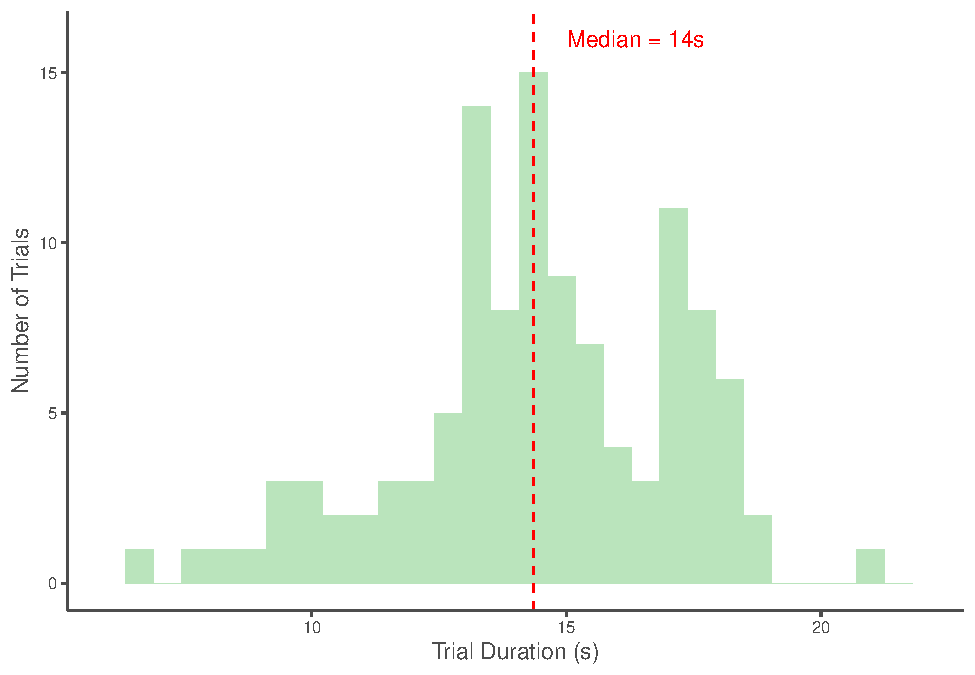
\includegraphics{revised_ms_analyses_files/figure-latex/r2-g-durations-trial-1.pdf}

\begin{Shaded}
\begin{Highlighting}[]
\FunctionTok{ggsave}\NormalTok{(}\FunctionTok{here}\NormalTok{(}\StringTok{\textquotesingle{}supplement/plots/exp\_2/pdfs\textquotesingle{}}\NormalTok{, }\StringTok{\textquotesingle{}g\_trialdur\_histogram.pdf\textquotesingle{}}\NormalTok{), }
       \AttributeTok{device=}\StringTok{\textquotesingle{}pdf\textquotesingle{}}\NormalTok{, }\AttributeTok{width=}\FloatTok{2.5}\NormalTok{, }\AttributeTok{height=}\FloatTok{1.25}\NormalTok{, }\AttributeTok{units=}\StringTok{\textquotesingle{}in\textquotesingle{}}\NormalTok{, }\AttributeTok{scale=}\FloatTok{2.5}\NormalTok{)}
\FunctionTok{ggsave}\NormalTok{(}\FunctionTok{here}\NormalTok{(}\StringTok{\textquotesingle{}supplement/plots/exp\_2/pngs\textquotesingle{}}\NormalTok{, }\StringTok{\textquotesingle{}g\_trialdur\_histogram.png\textquotesingle{}}\NormalTok{),}
       \AttributeTok{device=}\StringTok{\textquotesingle{}png\textquotesingle{}}\NormalTok{, }\AttributeTok{width=}\FloatTok{2.5}\NormalTok{, }\AttributeTok{height=}\FloatTok{1.25}\NormalTok{, }\AttributeTok{units=}\StringTok{\textquotesingle{}in\textquotesingle{}}\NormalTok{, }\AttributeTok{scale=}\FloatTok{2.5}\NormalTok{)}
\end{Highlighting}
\end{Shaded}

\begin{Shaded}
\begin{Highlighting}[]
\NormalTok{G\_MED\_TRIAL\_LOOKING\_S }\OtherTok{\textless{}{-}} \FunctionTok{median}\NormalTok{(}
\NormalTok{  g\_fin}\SpecialCharTok{$}\NormalTok{totaltrialtime\_looking\_sum\_s)}
\NormalTok{G\_MIN\_TRIAL\_LOOKING\_S }\OtherTok{\textless{}{-}} 
  \FunctionTok{min}\NormalTok{(g\_fin}\SpecialCharTok{$}\NormalTok{totaltrialtime\_looking\_sum\_s)}
\NormalTok{G\_MAX\_TRIAL\_LOOKING\_S }\OtherTok{\textless{}{-}} 
  \FunctionTok{max}\NormalTok{(g\_fin}\SpecialCharTok{$}\NormalTok{totaltrialtime\_looking\_sum\_s)}
\NormalTok{G\_MEAN\_TRIAL\_LOOKING\_S }\OtherTok{\textless{}{-}} 
  \FunctionTok{mean}\NormalTok{(g\_fin}\SpecialCharTok{$}\NormalTok{totaltrialtime\_looking\_sum\_s)}
\NormalTok{G\_CIL\_TRIAL\_LOOKING\_S }\OtherTok{\textless{}{-}}\NormalTok{ G\_MEAN\_TRIAL\_LOOKING\_S }\SpecialCharTok{{-}} 
  \FunctionTok{ci.low}\NormalTok{(g\_fin}\SpecialCharTok{$}\NormalTok{totaltrialtime\_looking\_sum\_s)}
\NormalTok{G\_CIH\_TRIAL\_LOOKING\_S }\OtherTok{\textless{}{-}}\NormalTok{ G\_MEAN\_TRIAL\_LOOKING\_S }\SpecialCharTok{+} 
  \FunctionTok{ci.high}\NormalTok{(g\_fin}\SpecialCharTok{$}\NormalTok{totaltrialtime\_looking\_sum\_s)}

\FunctionTok{ggplot}\NormalTok{(g\_fin, }\FunctionTok{aes}\NormalTok{(}\AttributeTok{x=}\NormalTok{totaltrialtime\_looking\_sum\_s)) }\SpecialCharTok{+}
  \FunctionTok{geom\_histogram}\NormalTok{(}\AttributeTok{fill=}\StringTok{"\#7bccc4"}\NormalTok{) }\SpecialCharTok{+}
\NormalTok{  sb.density.theme }\SpecialCharTok{+}
  \FunctionTok{geom\_vline}\NormalTok{(}\AttributeTok{xintercept=}\NormalTok{G\_MED\_TRIAL\_LOOKING\_S, }
             \AttributeTok{color=}\StringTok{"red"}\NormalTok{, }\AttributeTok{lty=}\DecValTok{2}\NormalTok{) }\SpecialCharTok{+}
  \FunctionTok{xlim}\NormalTok{(}\DecValTok{2}\NormalTok{,}\DecValTok{20}\NormalTok{) }\SpecialCharTok{+}
  \FunctionTok{xlab}\NormalTok{(}\StringTok{"Total Looking Time Duration (s)"}\NormalTok{) }\SpecialCharTok{+}
  \FunctionTok{ylab}\NormalTok{(}\StringTok{"Number of Trials"}\NormalTok{) }\SpecialCharTok{+} 
  \FunctionTok{theme}\NormalTok{(}\AttributeTok{axis.title =} \FunctionTok{element\_text}\NormalTok{(}\AttributeTok{colour=}\StringTok{"gray30"}\NormalTok{, }\AttributeTok{size=}\DecValTok{11}\NormalTok{),}
        \AttributeTok{axis.text =} \FunctionTok{element\_text}\NormalTok{(}\AttributeTok{colour=}\StringTok{"gray30"}\NormalTok{, }\AttributeTok{size=}\DecValTok{11}\NormalTok{),}
        \AttributeTok{axis.ticks =} \FunctionTok{element\_line}\NormalTok{(}\AttributeTok{colour=}\StringTok{"gray30"}\NormalTok{),}
        \AttributeTok{plot.background =} \FunctionTok{element\_blank}\NormalTok{(),}
        \AttributeTok{panel.grid.major =} \FunctionTok{element\_blank}\NormalTok{(),}
        \AttributeTok{panel.grid.minor =} \FunctionTok{element\_blank}\NormalTok{(),}
        \AttributeTok{panel.border =} \FunctionTok{element\_blank}\NormalTok{(),}
        \AttributeTok{panel.background =} \FunctionTok{element\_blank}\NormalTok{(),}
        \AttributeTok{axis.line =} \FunctionTok{element\_line}\NormalTok{(}\AttributeTok{color =} \StringTok{"gray30"}\NormalTok{))  }\SpecialCharTok{+}
  \FunctionTok{annotate}\NormalTok{(}
    \StringTok{"text"}\NormalTok{, }\AttributeTok{label =} \StringTok{"Median = 12s"}\NormalTok{,}
    \AttributeTok{x =}\NormalTok{ G\_MED\_TRIAL\_LOOKING\_S}\FloatTok{+2.5}\NormalTok{, }\AttributeTok{y =} \DecValTok{12}\NormalTok{, }\AttributeTok{size =} \DecValTok{4}\NormalTok{, }\AttributeTok{colour =} \StringTok{"red"}\NormalTok{)}
\end{Highlighting}
\end{Shaded}

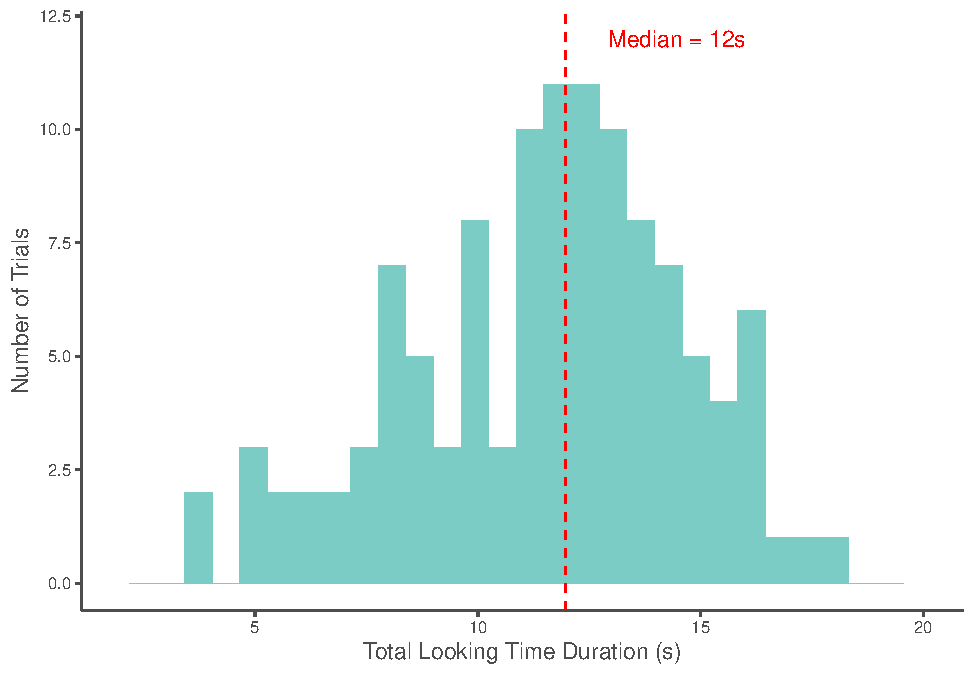
\includegraphics{revised_ms_analyses_files/figure-latex/r2-g-durations-triallooking-1.pdf}

\begin{Shaded}
\begin{Highlighting}[]
\FunctionTok{ggsave}\NormalTok{(}\FunctionTok{here}\NormalTok{(}\StringTok{\textquotesingle{}supplement/plots/exp\_2/pdfs\textquotesingle{}}\NormalTok{, }\StringTok{\textquotesingle{}g\_lookingtime\_histogram.pdf\textquotesingle{}}\NormalTok{), }
       \AttributeTok{device=}\StringTok{\textquotesingle{}pdf\textquotesingle{}}\NormalTok{, }\AttributeTok{width=}\FloatTok{2.5}\NormalTok{, }\AttributeTok{height=}\FloatTok{1.25}\NormalTok{, }\AttributeTok{units=}\StringTok{\textquotesingle{}in\textquotesingle{}}\NormalTok{, }\AttributeTok{scale=}\FloatTok{2.5}\NormalTok{)}
\FunctionTok{ggsave}\NormalTok{(}\FunctionTok{here}\NormalTok{(}\StringTok{\textquotesingle{}supplement/plots/exp\_2/pngs\textquotesingle{}}\NormalTok{, }\StringTok{\textquotesingle{}g\_lookingtime\_histogram.png\textquotesingle{}}\NormalTok{),}
       \AttributeTok{device=}\StringTok{\textquotesingle{}png\textquotesingle{}}\NormalTok{, }\AttributeTok{width=}\FloatTok{2.5}\NormalTok{, }\AttributeTok{height=}\FloatTok{1.25}\NormalTok{, }\AttributeTok{units=}\StringTok{\textquotesingle{}in\textquotesingle{}}\NormalTok{, }\AttributeTok{scale=}\FloatTok{2.5}\NormalTok{)}
\end{Highlighting}
\end{Shaded}

\begin{Shaded}
\begin{Highlighting}[]
\NormalTok{G\_MED\_LOOKING\_PROP }\OtherTok{\textless{}{-}} \FunctionTok{median}\NormalTok{(}
\NormalTok{  g\_fin}\SpecialCharTok{$}\NormalTok{trialtolookingoffset\_prop)}
\NormalTok{G\_MIN\_LOOKING\_PROP }\OtherTok{\textless{}{-}} \FunctionTok{min}\NormalTok{(}
\NormalTok{  g\_fin}\SpecialCharTok{$}\NormalTok{trialtolookingoffset\_prop)}
\NormalTok{G\_MAX\_LOOKING\_PROP }\OtherTok{\textless{}{-}} \FunctionTok{max}\NormalTok{(}
\NormalTok{  g\_fin}\SpecialCharTok{$}\NormalTok{trialtolookingoffset\_prop)}
\NormalTok{G\_MEAN\_LOOKING\_PROP }\OtherTok{\textless{}{-}} \FunctionTok{mean}\NormalTok{(}
\NormalTok{  g\_fin}\SpecialCharTok{$}\NormalTok{trialtolookingoffset\_prop)}
\NormalTok{G\_CIL\_LOOKING\_PROP }\OtherTok{\textless{}{-}}\NormalTok{ G\_MEAN\_LOOKING\_PROP }\SpecialCharTok{{-}} 
  \FunctionTok{ci.low}\NormalTok{(g\_fin}\SpecialCharTok{$}\NormalTok{trialtolookingoffset\_prop)}
\NormalTok{G\_CIH\_LOOKING\_PROP }\OtherTok{\textless{}{-}}\NormalTok{ G\_MEAN\_LOOKING\_PROP }\SpecialCharTok{+} 
  \FunctionTok{ci.high}\NormalTok{(g\_fin}\SpecialCharTok{$}\NormalTok{trialtolookingoffset\_prop)}

\FunctionTok{ggplot}\NormalTok{(g\_fin, }\FunctionTok{aes}\NormalTok{(}\AttributeTok{x=}\NormalTok{trialtolookingoffset\_prop)) }\SpecialCharTok{+}
  \FunctionTok{geom\_histogram}\NormalTok{(}\AttributeTok{fill=}\StringTok{"\#7bccc4"}\NormalTok{) }\SpecialCharTok{+}
\NormalTok{  sb.density.theme }\SpecialCharTok{+}
  \FunctionTok{geom\_vline}\NormalTok{(}\AttributeTok{xintercept=}\NormalTok{G\_MED\_LOOKING\_PROP, }\AttributeTok{color=}\StringTok{"red"}\NormalTok{, }\AttributeTok{lty=}\DecValTok{2}\NormalTok{) }\SpecialCharTok{+}
  \FunctionTok{xlim}\NormalTok{(}\DecValTok{0}\NormalTok{,}\DecValTok{1}\NormalTok{) }\SpecialCharTok{+}
  \FunctionTok{xlab}\NormalTok{(}\StringTok{"Overall Looking Time Proportion"}\NormalTok{) }\SpecialCharTok{+}
  \FunctionTok{ylab}\NormalTok{(}\StringTok{"Number of Trials"}\NormalTok{) }\SpecialCharTok{+} 
  \FunctionTok{theme}\NormalTok{(}\AttributeTok{axis.title =} \FunctionTok{element\_text}\NormalTok{(}\AttributeTok{colour=}\StringTok{"gray30"}\NormalTok{, }\AttributeTok{size=}\DecValTok{11}\NormalTok{),}
        \AttributeTok{axis.text =} \FunctionTok{element\_text}\NormalTok{(}\AttributeTok{colour=}\StringTok{"gray30"}\NormalTok{, }\AttributeTok{size=}\DecValTok{11}\NormalTok{),}
        \AttributeTok{axis.ticks =} \FunctionTok{element\_line}\NormalTok{(}\AttributeTok{colour=}\StringTok{"gray30"}\NormalTok{),}
        \AttributeTok{plot.background =} \FunctionTok{element\_blank}\NormalTok{() ,}
        \AttributeTok{panel.grid.major =} \FunctionTok{element\_blank}\NormalTok{() ,}
        \AttributeTok{panel.grid.minor =} \FunctionTok{element\_blank}\NormalTok{() ,}
        \AttributeTok{panel.border =} \FunctionTok{element\_blank}\NormalTok{() ,}
        \AttributeTok{panel.background =} \FunctionTok{element\_blank}\NormalTok{(),}
        \AttributeTok{axis.line =} \FunctionTok{element\_line}\NormalTok{(}\AttributeTok{color =} \StringTok{"gray30"}\NormalTok{)) }\SpecialCharTok{+}
  \FunctionTok{annotate}\NormalTok{(}
    \StringTok{"text"}\NormalTok{, }\AttributeTok{label =} \StringTok{"Median = 0.85"}\NormalTok{,}
    \AttributeTok{x =}\NormalTok{ G\_MED\_LOOKING\_PROP}\FloatTok{{-}.12}\NormalTok{, }\AttributeTok{y =} \DecValTok{16}\NormalTok{, }\AttributeTok{size =} \DecValTok{4}\NormalTok{, }\AttributeTok{colour =} \StringTok{"red"}\NormalTok{)}
\end{Highlighting}
\end{Shaded}

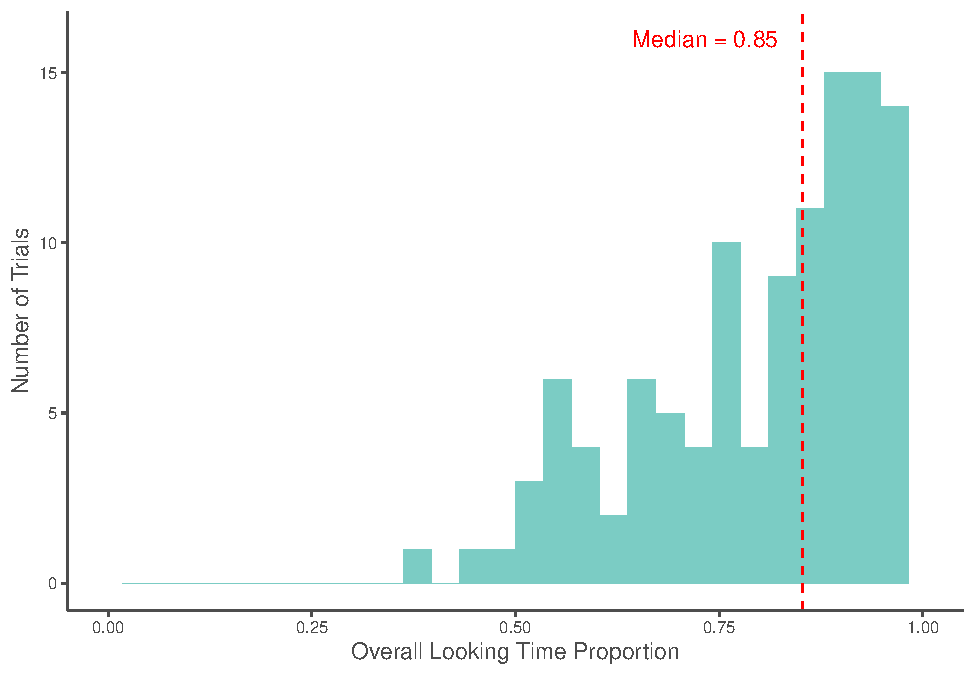
\includegraphics{revised_ms_analyses_files/figure-latex/r2-g-durs-lookingprop-1.pdf}

\begin{Shaded}
\begin{Highlighting}[]
\FunctionTok{ggsave}\NormalTok{(}\FunctionTok{here}\NormalTok{(}\StringTok{\textquotesingle{}supplement/plots/exp\_2/pdfs\textquotesingle{}}\NormalTok{, }\StringTok{\textquotesingle{}g\_lookingprop\_histogram.pdf\textquotesingle{}}\NormalTok{), }
       \AttributeTok{device=}\StringTok{\textquotesingle{}pdf\textquotesingle{}}\NormalTok{, }\AttributeTok{width=}\FloatTok{2.5}\NormalTok{, }\AttributeTok{height=}\FloatTok{1.25}\NormalTok{, }\AttributeTok{units=}\StringTok{\textquotesingle{}in\textquotesingle{}}\NormalTok{, }\AttributeTok{scale=}\FloatTok{2.5}\NormalTok{)}
\FunctionTok{ggsave}\NormalTok{(}\FunctionTok{here}\NormalTok{(}\StringTok{\textquotesingle{}supplement/plots/exp\_2/pngs\textquotesingle{}}\NormalTok{, }\StringTok{\textquotesingle{}g\_lookingprop\_histogram.png\textquotesingle{}}\NormalTok{),}
       \AttributeTok{device=}\StringTok{\textquotesingle{}png\textquotesingle{}}\NormalTok{, }\AttributeTok{width=}\FloatTok{2.5}\NormalTok{, }\AttributeTok{height=}\FloatTok{1.25}\NormalTok{, }\AttributeTok{units=}\StringTok{\textquotesingle{}in\textquotesingle{}}\NormalTok{, }\AttributeTok{scale=}\FloatTok{2.5}\NormalTok{)}
\end{Highlighting}
\end{Shaded}

\begin{Shaded}
\begin{Highlighting}[]
\NormalTok{G\_MED\_PRE\_DUR\_S }\OtherTok{\textless{}{-}} \FunctionTok{median}\NormalTok{(g\_fin}\SpecialCharTok{$}\NormalTok{pre\_dur\_ms}\SpecialCharTok{/}\DecValTok{1000}\NormalTok{)}
\NormalTok{G\_MIN\_PRE\_DUR\_S }\OtherTok{\textless{}{-}} \FunctionTok{min}\NormalTok{(g\_fin}\SpecialCharTok{$}\NormalTok{pre\_dur\_ms}\SpecialCharTok{/}\DecValTok{1000}\NormalTok{)}
\NormalTok{G\_MAX\_PRE\_DUR\_S }\OtherTok{\textless{}{-}} \FunctionTok{max}\NormalTok{(g\_fin[g\_fin}\SpecialCharTok{$}\NormalTok{pre\_dur\_ms}\SpecialCharTok{\textless{}}\DecValTok{10000}\NormalTok{,]}\SpecialCharTok{$}\NormalTok{pre\_dur\_ms}\SpecialCharTok{/}\DecValTok{1000}\NormalTok{)}
\NormalTok{G\_MEAN\_PRE\_DUR\_S }\OtherTok{\textless{}{-}} \FunctionTok{mean}\NormalTok{(g\_fin[g\_fin}\SpecialCharTok{$}\NormalTok{pre\_dur\_ms}\SpecialCharTok{\textless{}}\DecValTok{10000}\NormalTok{,]}\SpecialCharTok{$}\NormalTok{pre\_dur\_ms}\SpecialCharTok{/}\DecValTok{1000}\NormalTok{)}

\FunctionTok{ggplot}\NormalTok{(g\_fin, }\FunctionTok{aes}\NormalTok{(}\AttributeTok{x=}\NormalTok{pre\_dur\_ms}\SpecialCharTok{/}\DecValTok{1000}\NormalTok{))}\SpecialCharTok{+}
  \FunctionTok{geom\_histogram}\NormalTok{(}\AttributeTok{fill=}\StringTok{"\#bae4bc"}\NormalTok{) }\SpecialCharTok{+}
\NormalTok{  sb.density.theme }\SpecialCharTok{+}
  \FunctionTok{geom\_vline}\NormalTok{(}\AttributeTok{xintercept=}\NormalTok{G\_MED\_PRE\_DUR\_S, }\AttributeTok{color=}\StringTok{"red"}\NormalTok{, }\AttributeTok{lty=}\DecValTok{2}\NormalTok{) }\SpecialCharTok{+}
  \FunctionTok{xlim}\NormalTok{(}\DecValTok{2}\NormalTok{,}\FloatTok{6.5}\NormalTok{)}\SpecialCharTok{+}
  \FunctionTok{xlab}\NormalTok{(}\StringTok{\textquotesingle{}"Pre{-}Naming" Window Duration (s)\textquotesingle{}}\NormalTok{) }\SpecialCharTok{+}
  \FunctionTok{ylab}\NormalTok{(}\StringTok{"Number of Trials"}\NormalTok{) }\SpecialCharTok{+} 
  \FunctionTok{theme}\NormalTok{(}\AttributeTok{axis.title =} \FunctionTok{element\_text}\NormalTok{(}\AttributeTok{colour=}\StringTok{"gray30"}\NormalTok{, }\AttributeTok{size=}\DecValTok{11}\NormalTok{),}
        \AttributeTok{axis.ticks =} \FunctionTok{element\_line}\NormalTok{(}\AttributeTok{colour=}\StringTok{"gray30"}\NormalTok{),}
        \AttributeTok{plot.background =} \FunctionTok{element\_blank}\NormalTok{() ,}
        \AttributeTok{panel.grid.major =} \FunctionTok{element\_blank}\NormalTok{() ,}
        \AttributeTok{panel.grid.minor =} \FunctionTok{element\_blank}\NormalTok{() ,}
        \AttributeTok{panel.border =} \FunctionTok{element\_blank}\NormalTok{() ,}
        \AttributeTok{panel.background =} \FunctionTok{element\_blank}\NormalTok{(),}
        \AttributeTok{axis.line =} \FunctionTok{element\_line}\NormalTok{(}\AttributeTok{color =} \StringTok{"gray30"}\NormalTok{)) }\SpecialCharTok{+}
  \FunctionTok{annotate}\NormalTok{(}
    \StringTok{"text"}\NormalTok{, }\AttributeTok{label =} \StringTok{"Median = 3.5s"}\NormalTok{,}
    \AttributeTok{x =}\NormalTok{ G\_MED\_PRE\_DUR\_S}\FloatTok{+2.4}\NormalTok{, }\AttributeTok{y =} \DecValTok{25}\NormalTok{, }\AttributeTok{size =} \DecValTok{4}\NormalTok{, }\AttributeTok{colour =} \StringTok{"red"}\NormalTok{)}
\end{Highlighting}
\end{Shaded}

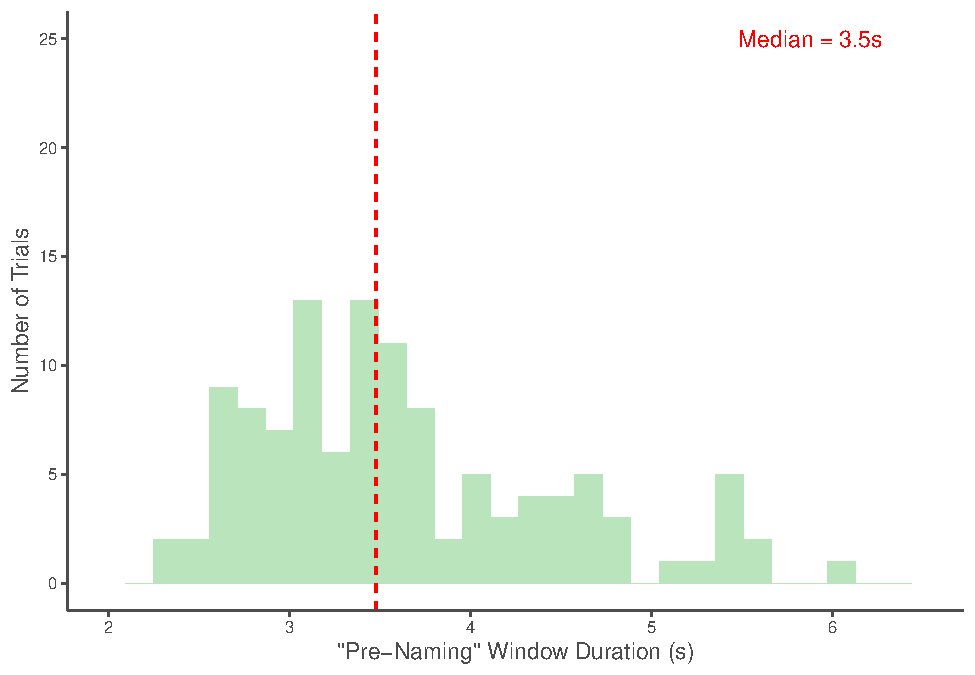
\includegraphics{revised_ms_analyses_files/figure-latex/r2-g-pre-duration-1.pdf}

\begin{Shaded}
\begin{Highlighting}[]
\NormalTok{g\_prelookingdur\_df }\OtherTok{\textless{}{-}}\NormalTok{ g\_fin }\SpecialCharTok{\%\textgreater{}\%} 
  \FunctionTok{mutate}\NormalTok{(}\AttributeTok{window =} \StringTok{\textquotesingle{}"Pre{-}Naming" Window\textquotesingle{}}\NormalTok{,}
         \AttributeTok{looking\_dur =}\NormalTok{ pre\_looking\_sum\_ms}\SpecialCharTok{/}\DecValTok{1000}\NormalTok{,}
         \AttributeTok{median =} \FunctionTok{median}\NormalTok{(looking\_dur),}
         \AttributeTok{mean =} \FunctionTok{mean}\NormalTok{(looking\_dur)) }\SpecialCharTok{\%\textgreater{}\%}
\NormalTok{  dplyr}\SpecialCharTok{::}\FunctionTok{select}\NormalTok{(}\StringTok{"subject\_id"}\NormalTok{, }\StringTok{"window"}\NormalTok{, }\StringTok{"looking\_dur"}\NormalTok{, }\StringTok{"median"}\NormalTok{, }\StringTok{"mean"}\NormalTok{)}

\NormalTok{G\_PRE\_MIN\_DUR }\OtherTok{\textless{}{-}} \FunctionTok{min}\NormalTok{(g\_prelookingdur\_df}\SpecialCharTok{$}\NormalTok{looking\_dur)}
\NormalTok{G\_PRE\_MAX\_DUR }\OtherTok{\textless{}{-}} \FunctionTok{max}\NormalTok{(g\_prelookingdur\_df}\SpecialCharTok{$}\NormalTok{looking\_dur)}
\NormalTok{G\_PRE\_MEAN\_DUR }\OtherTok{\textless{}{-}} \FunctionTok{mean}\NormalTok{(g\_prelookingdur\_df}\SpecialCharTok{$}\NormalTok{looking\_dur)}
\NormalTok{G\_PRE\_MEDIAN\_DUR }\OtherTok{\textless{}{-}} \FunctionTok{median}\NormalTok{(g\_prelookingdur\_df}\SpecialCharTok{$}\NormalTok{looking\_dur)}

\NormalTok{g\_postlookingdur\_df }\OtherTok{\textless{}{-}}\NormalTok{ g\_fin }\SpecialCharTok{\%\textgreater{}\%} 
  \FunctionTok{mutate}\NormalTok{(}\AttributeTok{window =} \StringTok{\textquotesingle{}"Post{-}Naming"/Analysis Window\textquotesingle{}}\NormalTok{,}
         \AttributeTok{looking\_dur =}\NormalTok{ post1\_looking\_sum\_ms}\SpecialCharTok{/}\DecValTok{1000}\NormalTok{,}
         \AttributeTok{median =} \FunctionTok{median}\NormalTok{(looking\_dur),}
         \AttributeTok{mean =} \FunctionTok{mean}\NormalTok{(looking\_dur)) }\SpecialCharTok{\%\textgreater{}\%}
\NormalTok{  dplyr}\SpecialCharTok{::}\FunctionTok{select}\NormalTok{(}\StringTok{"subject\_id"}\NormalTok{, }\StringTok{"window"}\NormalTok{, }\StringTok{"looking\_dur"}\NormalTok{, }\StringTok{"median"}\NormalTok{, }\StringTok{"mean"}\NormalTok{)}

\NormalTok{G\_POST\_MIN\_DUR }\OtherTok{\textless{}{-}} \FunctionTok{min}\NormalTok{(g\_postlookingdur\_df}\SpecialCharTok{$}\NormalTok{looking\_dur)}
\NormalTok{G\_POST\_MAX\_DUR }\OtherTok{\textless{}{-}} \FunctionTok{max}\NormalTok{(g\_postlookingdur\_df}\SpecialCharTok{$}\NormalTok{looking\_dur)}
\NormalTok{G\_POST\_MEAN\_DUR }\OtherTok{\textless{}{-}} \FunctionTok{mean}\NormalTok{(g\_postlookingdur\_df}\SpecialCharTok{$}\NormalTok{looking\_dur)}
\NormalTok{G\_POST\_MEDIAN\_DUR }\OtherTok{\textless{}{-}} \FunctionTok{median}\NormalTok{(g\_postlookingdur\_df}\SpecialCharTok{$}\NormalTok{looking\_dur)}

\NormalTok{g\_prepost\_lookingdur\_df }\OtherTok{\textless{}{-}} \FunctionTok{rbind}\NormalTok{(g\_prelookingdur\_df, g\_postlookingdur\_df)}
\NormalTok{g\_prepost\_lookingdur\_df}\SpecialCharTok{$}\NormalTok{window }\OtherTok{\textless{}{-}} 
  \FunctionTok{factor}\NormalTok{(g\_prepost\_lookingdur\_df}\SpecialCharTok{$}\NormalTok{window, }\AttributeTok{levels=}\FunctionTok{c}\NormalTok{(}
    \StringTok{\textquotesingle{}"Pre{-}Naming" Window\textquotesingle{}}\NormalTok{,}\StringTok{\textquotesingle{}"Post{-}Naming"/Analysis Window\textquotesingle{}}\NormalTok{), }\AttributeTok{ordered=}\NormalTok{T) }

\NormalTok{g\_prepost\_lookingdur\_label\_df }\OtherTok{\textless{}{-}}\NormalTok{ g\_prepost\_lookingdur\_df }\SpecialCharTok{\%\textgreater{}\%}
  \FunctionTok{group\_by}\NormalTok{(window) }\SpecialCharTok{\%\textgreater{}\%}
  \FunctionTok{summarize}\NormalTok{(}\AttributeTok{median=}\FunctionTok{median}\NormalTok{(median),}
            \AttributeTok{label=}\FunctionTok{paste}\NormalTok{(}\StringTok{"Median ="}\NormalTok{, }\FunctionTok{round}\NormalTok{(median, }\DecValTok{2}\NormalTok{), }\AttributeTok{sep=}\StringTok{" "}\NormalTok{))}

\NormalTok{g\_pp\_durs }\OtherTok{\textless{}{-}} \FunctionTok{ggplot}\NormalTok{(g\_prepost\_lookingdur\_df, }\FunctionTok{aes}\NormalTok{(}\AttributeTok{x=}\NormalTok{looking\_dur)) }\SpecialCharTok{+}
  \FunctionTok{geom\_histogram}\NormalTok{(}\AttributeTok{fill=}\StringTok{"\#7bccc4"}\NormalTok{) }\SpecialCharTok{+}
\NormalTok{  sb.density.theme }\SpecialCharTok{+}
  \FunctionTok{geom\_vline}\NormalTok{(}\FunctionTok{aes}\NormalTok{(}\AttributeTok{xintercept=}\NormalTok{median), }\AttributeTok{color=}\StringTok{"red"}\NormalTok{, }\AttributeTok{lty=}\DecValTok{2}\NormalTok{) }\SpecialCharTok{+}
  \FunctionTok{xlim}\NormalTok{(}\DecValTok{0}\NormalTok{,}\DecValTok{5}\NormalTok{) }\SpecialCharTok{+}
  \FunctionTok{xlab}\NormalTok{(}\StringTok{"Looking Time Duration (s)"}\NormalTok{) }\SpecialCharTok{+}
  \FunctionTok{ylab}\NormalTok{(}\StringTok{"Number of Trials"}\NormalTok{) }\SpecialCharTok{+} 
  \FunctionTok{theme}\NormalTok{(}\AttributeTok{axis.title =} \FunctionTok{element\_text}\NormalTok{(}\AttributeTok{colour=}\StringTok{"gray30"}\NormalTok{, }\AttributeTok{size=}\DecValTok{11}\NormalTok{),}
        \AttributeTok{axis.text =} \FunctionTok{element\_text}\NormalTok{(}\AttributeTok{colour=}\StringTok{"gray30"}\NormalTok{, }\AttributeTok{size=}\DecValTok{11}\NormalTok{),}
        \AttributeTok{axis.ticks =} \FunctionTok{element\_line}\NormalTok{(}\AttributeTok{colour=}\StringTok{"gray30"}\NormalTok{),}
        \AttributeTok{plot.background =} \FunctionTok{element\_blank}\NormalTok{(),}
        \AttributeTok{strip.text.x =} \FunctionTok{element\_text}\NormalTok{(}\AttributeTok{colour=}\StringTok{"gray30"}\NormalTok{, }\AttributeTok{size=}\DecValTok{11}\NormalTok{))}\SpecialCharTok{+}
  \FunctionTok{facet\_wrap}\NormalTok{(}\SpecialCharTok{\textasciitilde{}}\NormalTok{window) }\SpecialCharTok{+}
  \FunctionTok{geom\_text}\NormalTok{(}\AttributeTok{data=}\NormalTok{g\_prepost\_lookingdur\_label\_df,}
            \FunctionTok{aes}\NormalTok{(}\AttributeTok{x=}\NormalTok{median}\FloatTok{{-}1.2}\NormalTok{, }\AttributeTok{label=}\NormalTok{label), }\AttributeTok{y=}\DecValTok{45}\NormalTok{, }
            \AttributeTok{color=}\StringTok{"red"}\NormalTok{, }\AttributeTok{size=}\DecValTok{4}\NormalTok{)}

\FunctionTok{ggsave}\NormalTok{(}\FunctionTok{here}\NormalTok{(}\StringTok{\textquotesingle{}supplement/plots/exp\_2/pdfs\textquotesingle{}}\NormalTok{, }\StringTok{\textquotesingle{}g\_lookingdurs\_prepost.pdf\textquotesingle{}}\NormalTok{), }
       \AttributeTok{device=}\StringTok{\textquotesingle{}pdf\textquotesingle{}}\NormalTok{, }\AttributeTok{width=}\FloatTok{2.75}\NormalTok{, }\AttributeTok{height=}\FloatTok{1.5}\NormalTok{, }\AttributeTok{units=}\StringTok{\textquotesingle{}in\textquotesingle{}}\NormalTok{, }\AttributeTok{scale=}\FloatTok{2.5}\NormalTok{)}
\FunctionTok{ggsave}\NormalTok{(}\FunctionTok{here}\NormalTok{(}\StringTok{\textquotesingle{}supplement/plots/exp\_2/pngs\textquotesingle{}}\NormalTok{, }\StringTok{\textquotesingle{}g\_lookingdurs\_prepost.png\textquotesingle{}}\NormalTok{), }
       \AttributeTok{device=}\StringTok{\textquotesingle{}png\textquotesingle{}}\NormalTok{, }\AttributeTok{width=}\FloatTok{2.75}\NormalTok{, }\AttributeTok{height=}\FloatTok{1.5}\NormalTok{, }\AttributeTok{units=}\StringTok{\textquotesingle{}in\textquotesingle{}}\NormalTok{, }\AttributeTok{scale=}\FloatTok{2.5}\NormalTok{)}
\end{Highlighting}
\end{Shaded}

\begin{Shaded}
\begin{Highlighting}[]
\NormalTok{g\_prelookingprop\_df }\OtherTok{\textless{}{-}}\NormalTok{ g\_fin }\SpecialCharTok{\%\textgreater{}\%} 
  \FunctionTok{mutate}\NormalTok{(}\AttributeTok{window =} \StringTok{\textquotesingle{}"Pre{-}Naming" Window\textquotesingle{}}\NormalTok{,}
         \AttributeTok{looking\_prop =}\NormalTok{ pre\_looking\_sum\_ms}\SpecialCharTok{/}\NormalTok{pre\_dur\_ms,}
         \AttributeTok{median =} \FunctionTok{median}\NormalTok{(looking\_prop),}
         \AttributeTok{mean =} \FunctionTok{mean}\NormalTok{(looking\_prop)) }\SpecialCharTok{\%\textgreater{}\%}
\NormalTok{  dplyr}\SpecialCharTok{::}\FunctionTok{select}\NormalTok{(}\StringTok{"subject\_id"}\NormalTok{, }\StringTok{"window"}\NormalTok{, }\StringTok{"looking\_prop"}\NormalTok{, }\StringTok{"median"}\NormalTok{, }\StringTok{"mean"}\NormalTok{)}

\NormalTok{G\_PRE\_MIN\_PROP }\OtherTok{\textless{}{-}} \FunctionTok{min}\NormalTok{(g\_prelookingprop\_df}\SpecialCharTok{$}\NormalTok{looking\_prop)}
\NormalTok{G\_PRE\_MAX\_PROP }\OtherTok{\textless{}{-}} \FunctionTok{max}\NormalTok{(g\_prelookingprop\_df}\SpecialCharTok{$}\NormalTok{looking\_prop)}
\NormalTok{G\_PRE\_MEAN\_PROP }\OtherTok{\textless{}{-}} \FunctionTok{mean}\NormalTok{(g\_prelookingprop\_df}\SpecialCharTok{$}\NormalTok{looking\_prop)}
\NormalTok{G\_PRE\_MEDIAN\_PROP }\OtherTok{\textless{}{-}} \FunctionTok{median}\NormalTok{(g\_prelookingprop\_df}\SpecialCharTok{$}\NormalTok{looking\_prop)}

\NormalTok{g\_postlookingprop\_df }\OtherTok{\textless{}{-}}\NormalTok{ g\_fin }\SpecialCharTok{\%\textgreater{}\%} 
  \FunctionTok{mutate}\NormalTok{(}\AttributeTok{window =} \StringTok{\textquotesingle{}"Post{-}Naming"/Analysis Window\textquotesingle{}}\NormalTok{,}
         \AttributeTok{looking\_prop =}\NormalTok{ post1\_looking\_sum\_ms}\SpecialCharTok{/}\NormalTok{post1\_dur\_ms,}
         \AttributeTok{median =} \FunctionTok{median}\NormalTok{(looking\_prop),}
         \AttributeTok{mean =} \FunctionTok{mean}\NormalTok{(looking\_prop)) }\SpecialCharTok{\%\textgreater{}\%}
\NormalTok{  dplyr}\SpecialCharTok{::}\FunctionTok{select}\NormalTok{(}\StringTok{"subject\_id"}\NormalTok{, }\StringTok{"window"}\NormalTok{, }\StringTok{"looking\_prop"}\NormalTok{, }\StringTok{"median"}\NormalTok{, }\StringTok{"mean"}\NormalTok{)}

\NormalTok{G\_POST\_MIN\_PROP }\OtherTok{\textless{}{-}} \FunctionTok{min}\NormalTok{(g\_postlookingprop\_df}\SpecialCharTok{$}\NormalTok{looking\_prop)}
\NormalTok{G\_POST\_MAX\_PROP }\OtherTok{\textless{}{-}} \FunctionTok{max}\NormalTok{(g\_postlookingprop\_df}\SpecialCharTok{$}\NormalTok{looking\_prop)}
\NormalTok{G\_POST\_MEAN\_PROP }\OtherTok{\textless{}{-}} \FunctionTok{mean}\NormalTok{(g\_postlookingprop\_df}\SpecialCharTok{$}\NormalTok{looking\_prop)}
\NormalTok{G\_POST\_MEDIAN\_PROP }\OtherTok{\textless{}{-}} \FunctionTok{median}\NormalTok{(g\_postlookingprop\_df}\SpecialCharTok{$}\NormalTok{looking\_prop)}

\NormalTok{g\_prepost\_lookingprop\_df }\OtherTok{\textless{}{-}} \FunctionTok{rbind}\NormalTok{(g\_prelookingprop\_df, g\_postlookingprop\_df)}
\NormalTok{g\_prepost\_lookingprop\_df}\SpecialCharTok{$}\NormalTok{window }\OtherTok{\textless{}{-}} 
  \FunctionTok{factor}\NormalTok{(g\_prepost\_lookingprop\_df}\SpecialCharTok{$}\NormalTok{window, }\AttributeTok{levels=}\FunctionTok{c}\NormalTok{(}
    \StringTok{\textquotesingle{}"Pre{-}Naming" Window\textquotesingle{}}\NormalTok{,}\StringTok{\textquotesingle{}"Post{-}Naming"/Analysis Window\textquotesingle{}}\NormalTok{), }\AttributeTok{ordered=}\NormalTok{T) }

\NormalTok{g\_prepost\_lookingprop\_label\_df }\OtherTok{\textless{}{-}}\NormalTok{ g\_prepost\_lookingprop\_df }\SpecialCharTok{\%\textgreater{}\%}
  \FunctionTok{group\_by}\NormalTok{(window) }\SpecialCharTok{\%\textgreater{}\%}
  \FunctionTok{summarize}\NormalTok{(}\AttributeTok{median=}\FunctionTok{median}\NormalTok{(median),}
            \AttributeTok{label=}\FunctionTok{paste}\NormalTok{(}\StringTok{"Median ="}\NormalTok{, }\FunctionTok{round}\NormalTok{(median, }\DecValTok{2}\NormalTok{), }\AttributeTok{sep=}\StringTok{" "}\NormalTok{))}

\FunctionTok{ggplot}\NormalTok{(g\_prepost\_lookingprop\_df, }\FunctionTok{aes}\NormalTok{(}\AttributeTok{x=}\NormalTok{looking\_prop)) }\SpecialCharTok{+}
  \FunctionTok{geom\_histogram}\NormalTok{(}\AttributeTok{fill=}\StringTok{"\#7bccc4"}\NormalTok{) }\SpecialCharTok{+}
\NormalTok{  sb.density.theme }\SpecialCharTok{+}
  \FunctionTok{geom\_vline}\NormalTok{(}\FunctionTok{aes}\NormalTok{(}\AttributeTok{xintercept=}\NormalTok{median), }\AttributeTok{color=}\StringTok{"red"}\NormalTok{, }\AttributeTok{lty=}\DecValTok{2}\NormalTok{) }\SpecialCharTok{+}
  \FunctionTok{xlim}\NormalTok{(}\DecValTok{0}\NormalTok{,}\DecValTok{1}\NormalTok{) }\SpecialCharTok{+}
  \FunctionTok{ylim}\NormalTok{(}\DecValTok{0}\NormalTok{,}\DecValTok{22}\NormalTok{) }\SpecialCharTok{+}
  \FunctionTok{xlab}\NormalTok{(}\StringTok{"Looking Time Proportion"}\NormalTok{) }\SpecialCharTok{+}
  \FunctionTok{ylab}\NormalTok{(}\StringTok{"Number of Trials"}\NormalTok{) }\SpecialCharTok{+} 
  \FunctionTok{theme}\NormalTok{(}\AttributeTok{axis.title =} \FunctionTok{element\_text}\NormalTok{(}\AttributeTok{colour=}\StringTok{"gray30"}\NormalTok{, }\AttributeTok{size=}\DecValTok{11}\NormalTok{),}
        \AttributeTok{axis.text =} \FunctionTok{element\_text}\NormalTok{(}\AttributeTok{colour=}\StringTok{"gray30"}\NormalTok{, }\AttributeTok{size=}\DecValTok{11}\NormalTok{),}
        \AttributeTok{axis.ticks =} \FunctionTok{element\_line}\NormalTok{(}\AttributeTok{colour=}\StringTok{"gray30"}\NormalTok{),}
        \AttributeTok{plot.background =} \FunctionTok{element\_blank}\NormalTok{(),}
        \AttributeTok{strip.text.x =} \FunctionTok{element\_text}\NormalTok{(}\AttributeTok{colour=}\StringTok{"gray30"}\NormalTok{, }\AttributeTok{size=}\DecValTok{11}\NormalTok{))}\SpecialCharTok{+}
  \FunctionTok{facet\_wrap}\NormalTok{(}\SpecialCharTok{\textasciitilde{}}\NormalTok{window) }\SpecialCharTok{+}
  \FunctionTok{geom\_text}\NormalTok{(}\AttributeTok{data=}\NormalTok{g\_prepost\_lookingprop\_label\_df,}
            \FunctionTok{aes}\NormalTok{(}\AttributeTok{x=}\NormalTok{median}\FloatTok{{-}.24}\NormalTok{, }\AttributeTok{label=}\NormalTok{label), }\AttributeTok{y=}\DecValTok{21}\NormalTok{, }
            \AttributeTok{color=}\StringTok{"red"}\NormalTok{, }\AttributeTok{size=}\DecValTok{4}\NormalTok{)}
\end{Highlighting}
\end{Shaded}

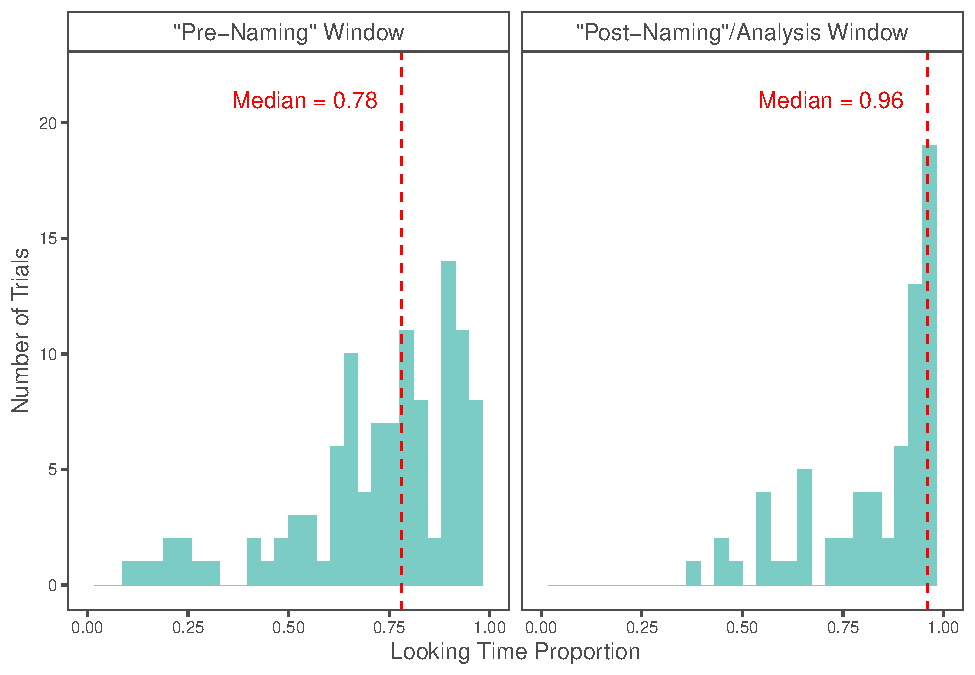
\includegraphics{revised_ms_analyses_files/figure-latex/r2-g-durs-prepost-lookingprops-1.pdf}

\begin{Shaded}
\begin{Highlighting}[]
\FunctionTok{ggsave}\NormalTok{(}\FunctionTok{here}\NormalTok{(}\StringTok{\textquotesingle{}supplement/plots/exp\_2/pdfs\textquotesingle{}}\NormalTok{, }\StringTok{\textquotesingle{}g\_lookingprops\_prepost.pdf\textquotesingle{}}\NormalTok{), }
       \AttributeTok{device=}\StringTok{\textquotesingle{}pdf\textquotesingle{}}\NormalTok{, }\AttributeTok{width=}\FloatTok{2.75}\NormalTok{, }\AttributeTok{height=}\FloatTok{1.5}\NormalTok{, }\AttributeTok{units=}\StringTok{\textquotesingle{}in\textquotesingle{}}\NormalTok{, }\AttributeTok{scale=}\FloatTok{2.5}\NormalTok{)}
\FunctionTok{ggsave}\NormalTok{(}\FunctionTok{here}\NormalTok{(}\StringTok{\textquotesingle{}supplement/plots/exp\_2/pngs\textquotesingle{}}\NormalTok{, }\StringTok{\textquotesingle{}g\_lookingprops\_prepost.png\textquotesingle{}}\NormalTok{), }
       \AttributeTok{device=}\StringTok{\textquotesingle{}png\textquotesingle{}}\NormalTok{, }\AttributeTok{width=}\FloatTok{2.75}\NormalTok{, }\AttributeTok{height=}\FloatTok{1.5}\NormalTok{, }\AttributeTok{units=}\StringTok{\textquotesingle{}in\textquotesingle{}}\NormalTok{, }\AttributeTok{scale=}\FloatTok{2.5}\NormalTok{)}
\end{Highlighting}
\end{Shaded}

Trials in Experiment 2 were \(14.29\)\textit{s} {[}\(13.74\), \(14.84\){]} long on average (\textit{range}: \(4.34-20.99\)\textit{s}, \textit{Med}\(=14.36\)\textit{s}), and infants spent an average of \(11.50\)\textit{s} {[}\(10.93\), \(12.05\){]} total looking at the displays (\textit{range}: \(3.43-18.15\)\textit{s}, \textit{Med}\(=11.96\)\textit{s}, or between \(0.39\) and \(1.00\) of the total trial duration; \(M=0.81\) {[}\(0.78\), \(0.83\){]}, \textit{Med}\(=0.85\)).

The pre-naming window was between \(2.31\) and \(6.12\)\textit{s} (\(M_\textnormal{pre}=3.63\)\textit{s}, \(Med_\textnormal{pre}=3.48\)\textit{s}).

The children in our final sample spent similar proportions of time looking at the displays during the pre- and post-naming periods (pre-naming: \(0.12-1\), \(M_\textnormal{proportion}=0.74\), \(Med_\textnormal{proportion}=0.78\); post-naming: \(0.38-1\), \(M_\textnormal{proportion}=0.90\), \(Med_\textnormal{proportion}=0.96\)).


\end{document}
